\chapter{An integrative `omics approach to quantitative analysis of physiological metabolic flux control\label{ch:simmer}}

\section{Abstract}

Enzyme and metabolite quantitation has been revolutionized by advances in mass spectrometry, but methods to integrate the resulting data remain needed. Here we present a quantitative, scalable strategy for revealing steady-state metabolic regulation by integration of metabolomic, proteomic, and flux measurements. It involves analyzing, on a reaction-by-reaction basis, whether fluxes across conditions are accounted for by a Michaelis-Menten relationship between enzyme, substrate, and potential regulator concentrations. We collected the required data for yeast growing at 25 different nutrients-limited steady states and applied this strategy to reveal the primary physiological flux control mechanisms for over 40 metabolic reactions, encompassing 32 instances of physiologically-relevant allosteric regulation. The identified regulation included classical feedbacks and unexpected cross-pathway connections. Quantitatively, half of flux control resided in substrate and one quarter in enzyme concentrations. For reversible reactions, the remainder resided largely in product levels, and for irreversible reactions in allosteric effectors. Thus, metabolic activity is substantially self-regulated by metabolites themselves.

\section{Introduction}

A crowning achievement of twentieth century biochemistry was determining the pathways by which organisms convert diverse nutrients into macromolecules \cite{Caspi:2014je}. Despite extensive knowledge of metabolic reaction networks, even in the best-studied model microbes, the means by which metabolic reaction rates (fluxes) are controlled remains incompletely understood. Specifically, while mechanisms controlling the expression and activity of many metabolic enzymes are known, how these multiple modes of regulation come together in cells to control reaction rates is largely unanswered.

Most metabolic regulatory mechanisms were discovered by isolating enzymes and studying their kinetics \textit{in vitro}. While powerful for proving specific regulatory interactions, this reductionist approach is less effective at revealing which mechanisms play a predominant role in cells. For example, the true impact of certain regulators may be evident only in the presence of physiologic concentrations of substrates and other metabolites \cite{Fell:1997wg, Tummler:2014cp}. Moreover, certain regulators may change only slightly in concentration across biological conditions and therefore matter relatively little, whereas others change greatly and thus dominate flux control \cite{Kacser:1973fe}. 

To rigorously understand control of metabolic fluxes in cells, quantitative analysis is critical. The framework of metabolic control analysis (MCA) uses flux control coefficients (C$^{J}_{E}$) to capture the importance of a given enzyme's concentration ([E]) to overall pathway flux (J), with C$^{J}_{E}$  = $(dJ/J)/(d[E]/[E])$ \cite{Kacser:1973fe}. Experimental determination of flux control coefficients is, however, difficult, and regulatory interactions in cells may result in flux being weakly linked to pathway enzymes \cite{Hauf:2000vu, Kochanowski:2013fb, Fell:1997wg, CornishBowden:1995fy}. For example, the rate of glycolytic flux may be determined by total cellular ATP demand rather than glycolytic enzyme expression \cite{Koebmann:2002ic}. Thus, there is a need for additional approaches to link available experimental data to flux control.

To this end, there has been growing interest in building differential equation models of metabolic dynamics. Each reaction is typically associated with multiple parameters (e.g., k$_{cat}$, k$_{m}$, k$_{i}$), with changes to the parameters describing any one reaction altering the entire system dynamics. By tuning enzyme kinetic parameters and sifting through possible regulators, such models can be fit to experimental metabolite concentration data \cite{Teusink:2000kc, Chassagnole:2002ty, Tummler:2014cp}. The difficulty is that parameter and regulator identification requires global non-linear search in high-dimensional space. Accordingly, parameter and regulator identification scales poorly with network size and missing prior knowledge. Therefore, there is a need for new approaches that scale to the genome-level and are adaptable to systems with limited prior knowledge.

Here we present an approach that we term Systematic Identification of Meaningful Metabolic Enzyme Regulation (SIMMER). By combining steady-state proteomic, metabolomic, and fluxomic data, SIMMER evaluates on a reaction-by-reaction basis the physiological mechanisms underlying flux control in a quantitative manner. Specifically, given measurements of fluxes, metabolites, and enzymes across multiple steady states, SIMMER tests, one reaction at a time, whether the observed fluxes can be explained by a Michaelis-Menten relationship between substrate, product, and enzyme concentrations (\hyperref[fig:schema]{Figure \ref{fig:schema}A}). When a misfit is observed, it then searches for potential regulators that significantly rectify the discrepancy (\hyperref[fig:schema]{Figure \ref{fig:schema}B}). Because parameters and regulators are identified one reaction at a time, the approach is scalable.

Here we report integrative �omic analysis of 25 different steady-state yeast growth conditions, and subsequent application of SIMMER to reveal metabolic regulation. SIMMER recapitulates much of known regulation and reveals novel regulation. In addition, it determines the quantitative fraction of regulation residing in substrate, product, enzyme, and allosteric effector concentrations.

\begin{figure}[h!]
\includegraphics[width=1\textwidth]{ch-simmer/Figures/F1-schema.pdf}
\caption[We can infer \textit{in vivo} reaction kinetics if we have measured the reaction's rate and concentrations of enzymes and all relevant substrates, products and effectors]{We can infer \textit{in vivo} reaction kinetics if we have measured the reaction's rate and concentrations of enzymes and all relevant substrates, products and effectors.  Using `omic methods, these quantities can be measured in a high-throughput manner, allowing the kinetics of many reactions to be inferred in parallel.  \textbf{A)} For reactions that follow simple Michaelis-Menten \textit{in vivo} kinetics, measurements of enzyme and substrate/product concentration should agree with measured flux.  \textbf{B)} For reactions with physiologically-meaningful allostery, this regulation must be added before flux can be accurately predicted.  If multiple regulatory candidates exist, better supported candidates will result in greater improvement in flux prediction.  For reactions where none of the tested regulators results in an accurate prediction of flux, other unaccounted for regulation may be kinetically important.}
\label{fig:schema}
\end{figure}

\section{Results}

\subsection{Systems-level metabolite and enzyme concentrations and fluxes.}

We determined fluxes, metabolite concentrations, and enzyme concentrations, across 25 different steady-state yeast cultures. Yeast were grown in chemostats limited for carbon, nitrogen, phosphorus, leucine, or uracil, each at five different growth rates. Carbon, nitrogen, and phosphorous limitation were implemented in prototrophic yeast through manipulation of the media glucose, ammonium, and phosphate, respectively; leucine and uracil limitation were implemented in auxotrophs. Collectively, these conditions span a broad range of yeast physiology and metabolism.

To determine fluxes across these conditions, we employed flux balance analysis constrained by experimental measurements of nutrient uptake, waste excretion, and biomass generation. Uptake of glucose (the sole carbon source) and excretion of waste products were measured by $^{1}$H-NMR (\hyperref[fig:boundFlux]{Figure \ref{fig:boundFlux}}). In addition, yeast composition was evaluated by measuring the fraction of protein, carbohydrate, RNA, DNA, polyphosphate, and fatty acids. Intriguingly, we observed notable differences in composition across conditions. This included, as expected based on prior literature \cite{Schulze:1995uv, Lange:2001th}, a strong positive correlation, irrespective of the limiting nutrient, between nucleic acid content (primarily in the form of ribosomal RNA) and growth rates, and a similar but less strong trend for total protein content. It also included differences across nutrient conditions, which were particularly evident at slow growth rate, including fat and polyphosphate accumulation in nitrogen limitation. Direct experimental determination of these differences in biomass was important for accurate flux determination, as the product of growth rate and fractional composition determines net biosynthetic fluxes (\hyperref[fig:boundFlux]{Figure \ref{fig:boundFlux}}).

The combined uptake, excretion, and biomass production fluxes effectively constrained intracellular fluxes, whose values were determined by flux balance analysis by optimizing fit to experimental data and minimizing total network flux \cite{Herrgard:2008gb, Yizhak:2010jk}. The range of fluxes that were equally compatible with these constraints was determined by flux variability analysis (see methods) \cite{Mahadevan:2003wq}. This approach allowed us to determine the fluxes of 233 metabolic reactions (\hyperref[fig:fluxHM]{Figure \ref{fig:fluxHM}}). With some important exceptions, such as more amino acid biosynthesis in leucine limitation and less glycolytic flux in glucose limitation, flux correlated strongly with growth rate.

The relative concentrations of 106 metabolites were previously measured across these chemostat conditions by LC-MS/MS \cite{Boer:2010fb}. Overall, metabolite abundances depended strongly on the nature of the limiting nutrient. Products made from the limiting nutrient, such as amino acids in nitrogen limitation and nucleotide triphosphates in phosphorous limitation, were strongly depleted at slow growth rate. In contrast, associated metabolites lacking the limiting element, such as $\alpha$-ketoglutarate in nitrogen limitation and nucleosides in phosphorous limitation, tended to accumulate. Here we augmented these observations based on relative measurements, with absolute measurements by an isotope ratio-based approach. From absolute concentration measurements for a single reference condition, we deduced absolute concentrations across all conditions. This enabled us to compare metabolite concentrations to biochemical measurements of enzyme site affinities. 

An isotope ratio-based LC-MS/MS approach was also used to analyze the proteome. To determine relative protein abundances across conditions, each experimental sample was compared to a common $^{15}$N-labeled internal reference sample \cite{Oda:1999uz,Ong:2002tf}. Quantitative data was obtained for over 20,000 peptides representing 1187 proteins. Repeat measurements comparing slow-growing nitrogen and phosphorus-limited chemostats showed good reproducibility (\hyperref[fig:proteomicsConsistency]{Figure \ref{fig:proteomicsConsistency}}). Unlike metabolites, the abundances of many proteins, especially ribosomal proteins, depended primarily on growth rate irrespective of the limiting nutrient (\hyperref[fig:proteinHM]{Figure \ref{fig:proteinHM}}). Quantitatively, the fraction of concentration variation explained by growth rate alone was greater for the proteome than the metabolome, but less than for the transcriptome (\hyperref[fig:dataSummary]{Figure \ref{fig:dataSummary}A}) \cite{Brauer:2008jn}.

The measured proteins included 370 metabolic enzymes, a number similar to that obtained by SRM-based approaches tailored for enzyme quantitation \cite{Costenoble:2011hia, Zampar:2013fr} (\hyperref[protTable]{Table \ref{protTable}}). Much like metabolite abundances, metabolic enzyme abundances varied strongly depending on the limiting nutrient. Compared to proteins overall, the relative concentrations of small molecule metabolic enzymes depended less on general growth rate and more on the specific limiting nutrient (\hyperref[fig:dataSummary]{Figure \ref{fig:dataSummary}A}). Notable nutrient-specific trends included down-regulation of glycolytic enzymes and up-regulation of TCA ones in carbon limitation, and increased levels of amino acid biosynthetic enzymes in leucine limitation (\hyperref[fig:dataSummary]{Figure \ref{fig:dataSummary}B}). Thus, relative to transcripts or proteins in general, the abundances of metabolites and metabolic enzymes are tied more strongly to the particular nutrient environment. In the case metabolites, this may directly reflect mass action, whereas for metabolic enzymes it may reflect regulation designed to maintain appropriate flux as nutrient and thus metabolite levels change.

In total, we obtained the requisite integrative `omics data (flux, enzyme concentration, substrate concentrations, and optionally product concentrations) for 56 reactions.

\begin{figure}[H]
\floatbox[{\capbeside\thisfloatsetup{capbesideposition={right,top},capbesidewidth=6cm}}]{figure}[\FBwidth]
{\caption[Summary of input data]{\fixedspaceword{Summary of input data. \textbf{A)} The relative impact of growth rate and limiting nutrients in driving systematic variation of transcripts, proteins, enzymes and metabolites was tested through comparison of nested regression models.  Proceeding from simpler to more complicated models, the fraction of variation explained across all genes/metabolites explained by the added term indicates its relative impact on abundance. \textbf{B)} Heatmap summarizing the variable concentration of 370 enzymes across chemostat conditions. From the ratio of unlabelled sample peptides to matching $^{15}N$-labelled reference peptides, the abundance of each enzyme relative to a common reference was determined.  Across the 25 conditions, enzyme relative abundances were mean-centered, log-transformed and organized by hierarchical clustering using pearson correlation with average linkage.
}}\label{fig:dataSummary}}
{\includegraphics[width=\textwidth-6cm]{ch-simmer/Figures/F2-DataSummary.pdf}}
\end{figure}

\subsection{Integration of concentration and flux data via SIMMER.}

Substrate, product, and enzyme concentrations can be related to flux through standard reversible Michaelis-Menten kinetics. For generality, a reversible rate law that assumes random-order enzyme mechanism and substrate/product competition was employed for all reactions \cite{Liebermeister:2006fm, Tummler:2014cp}. Kinetic parameters were identified by non-linear optimization to maximize the consistency of the Michaelis-Menten model and measured flux. 

As a first example, consider the triose-phosphate isomerase (TPI1) reaction in glycolysis which converts dihydroxyacetone phosphate (DHAP) into glyceraldehyde 3-phosophate (GAP). Concentrations of substrate and product varied largely in tandem across the 25 chemostat conditions, with a trend towards increasing levels of both with faster growth (\hyperref[fig:TPI]{Figure \ref{fig:TPI}A}). Tpi1p concentration was lowest in carbon limitation and did not vary strongly with growth rate, even though flux increased markedly with faster growth (\hyperref[fig:TPI]{Figure \ref{fig:TPI}A,B}). As substrate concentration generally tracked with flux, and low Tpi1p concentrations aligned with the low glycolytic flux in carbon limitation, integration of these data via SIMMER, without invoking any overt regulation, was sufficient to explain most of the flux variability across the 25 conditions. 

\begin{figure}[h!]
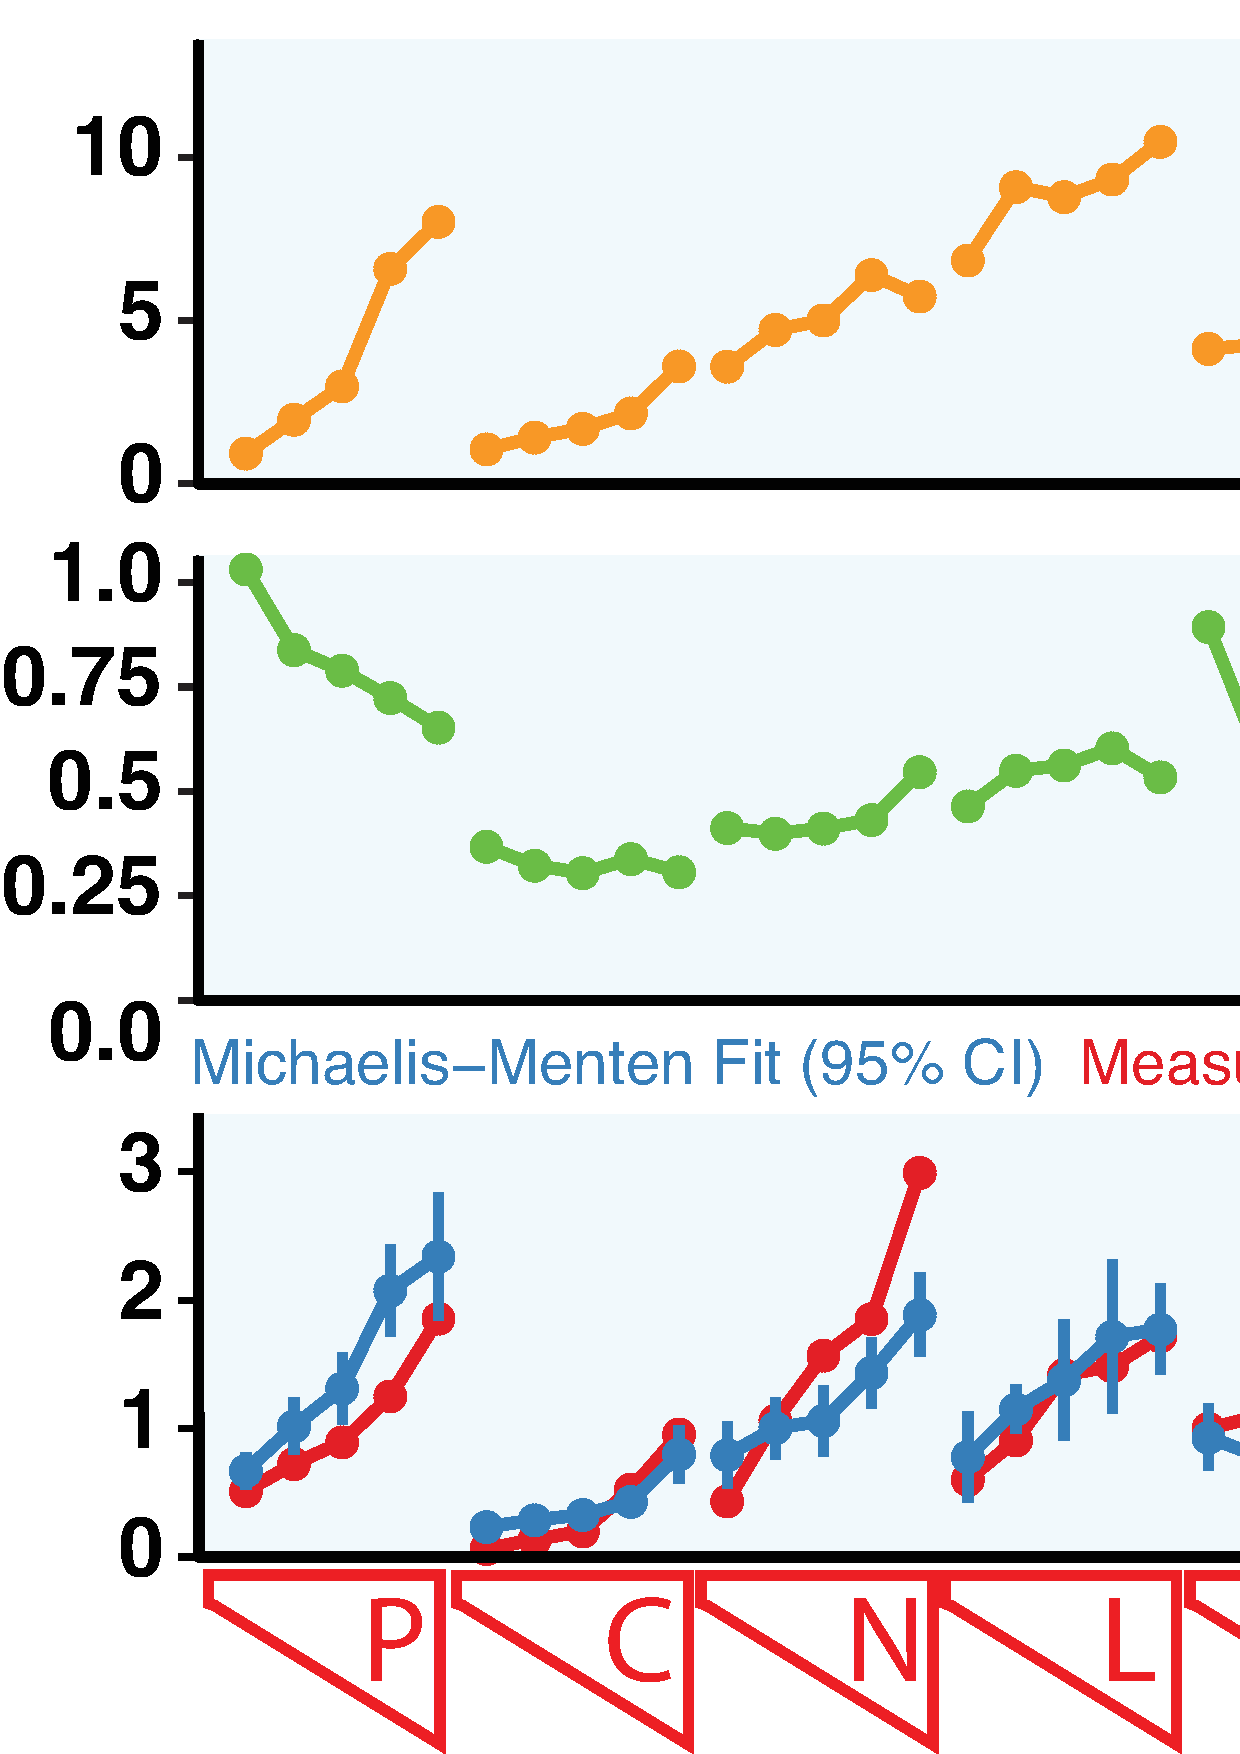
\includegraphics[width = 1\textwidth]{ch-simmer/Figures/F3-MMkinetics.pdf}
\caption[Michaelis-Menten kinetics is sufficient to relate substrate, product and enzyme concentrations to flux carried for the reaction triose-phosphate isomerase]{Michaelis-Menten kinetics is sufficient to relate substrate, product and enzyme concentrations to flux carried for the reaction triose-phosphate isomerase.  \textbf{A)} Across 25 conditions, we measured the relative concentration the reaction substrate (DHAP: dihydroxyacetone phosphate), product (GA3P: glyceraldehyde 3-phosphate) and enzyme (TPI: Tpi1).  \textbf{B)} The simple Michaelis-Menten reaction form translates the 25 sets of reaction species into predict flux ($V_{rMM}$) based on the value of four inferred kinetic parameters.  Comparing measured flux to the reaction form's prediction indicates that flux through TPI can be explained by a Michaelis-Menten relationship between substrate, product and enzyme.}
\label{fig:TPI}
\end{figure}

The same approach was used to study amidophosphoribosyltransferase (ADE4), the first committed step of purine biosynthesis. Both of the substrates of this reaction were strongly influenced by limiting nutrient, with PRPP specifically-depleted in phosphate limitation and glutamine in nitrogen limitation; the product glutamate was most abundant in carbon limitation (\hyperref[fig:PPAT]{Figure \ref{fig:PPAT}A}; phosphoribosylamine was not measured). Ade4p enzyme concentration was lowest in carbon limitation and greatest in leucine limitation. From these patterns of substrate, product, and enzyme concentrations, it was possible to account for only half the observed variation across conditions in fluxes, which increased more with growth rate than could be accounted for based on the measured concentrations (\hyperref[fig:PPAT]{Figure \ref{fig:PPAT}B}). To determine whether allosteric regulation could rectify this inconsistency, we compiled a list of nine candidate activators and inhibitors from the BRENDA database, drawing upon both both yeast-specific regulation and non-yeast regulation spanning all domains of life \cite{Scheer:2011df}. For each, the corresponding Michaelis-Menten rate law was evaluated for whether it explained the observed flux significantly better than the regulation-free rate law (q-value $<$ 0.1). Of the nine, only inhibition by adenosine monophosphate (AMP), which generally accumulates in slow growth, meaningfully improved fit (\hyperref[fig:PPAT]{Figure \ref{fig:PPAT}C}). Inhibition of the first committed step of purine biosynthesis by AMP is a logical feedback circuit that has been demonstrated in yeast and in other organisms \cite{WYNGAARDEN:1959wf, Jones:1982dn}. Thus, from a set of candidates based on prior knowledge of metabolism, SIMMER was able to identify physiologically relevant allosteric regulation of yeast purine biosynthesis.

\begin{figure}[h!]
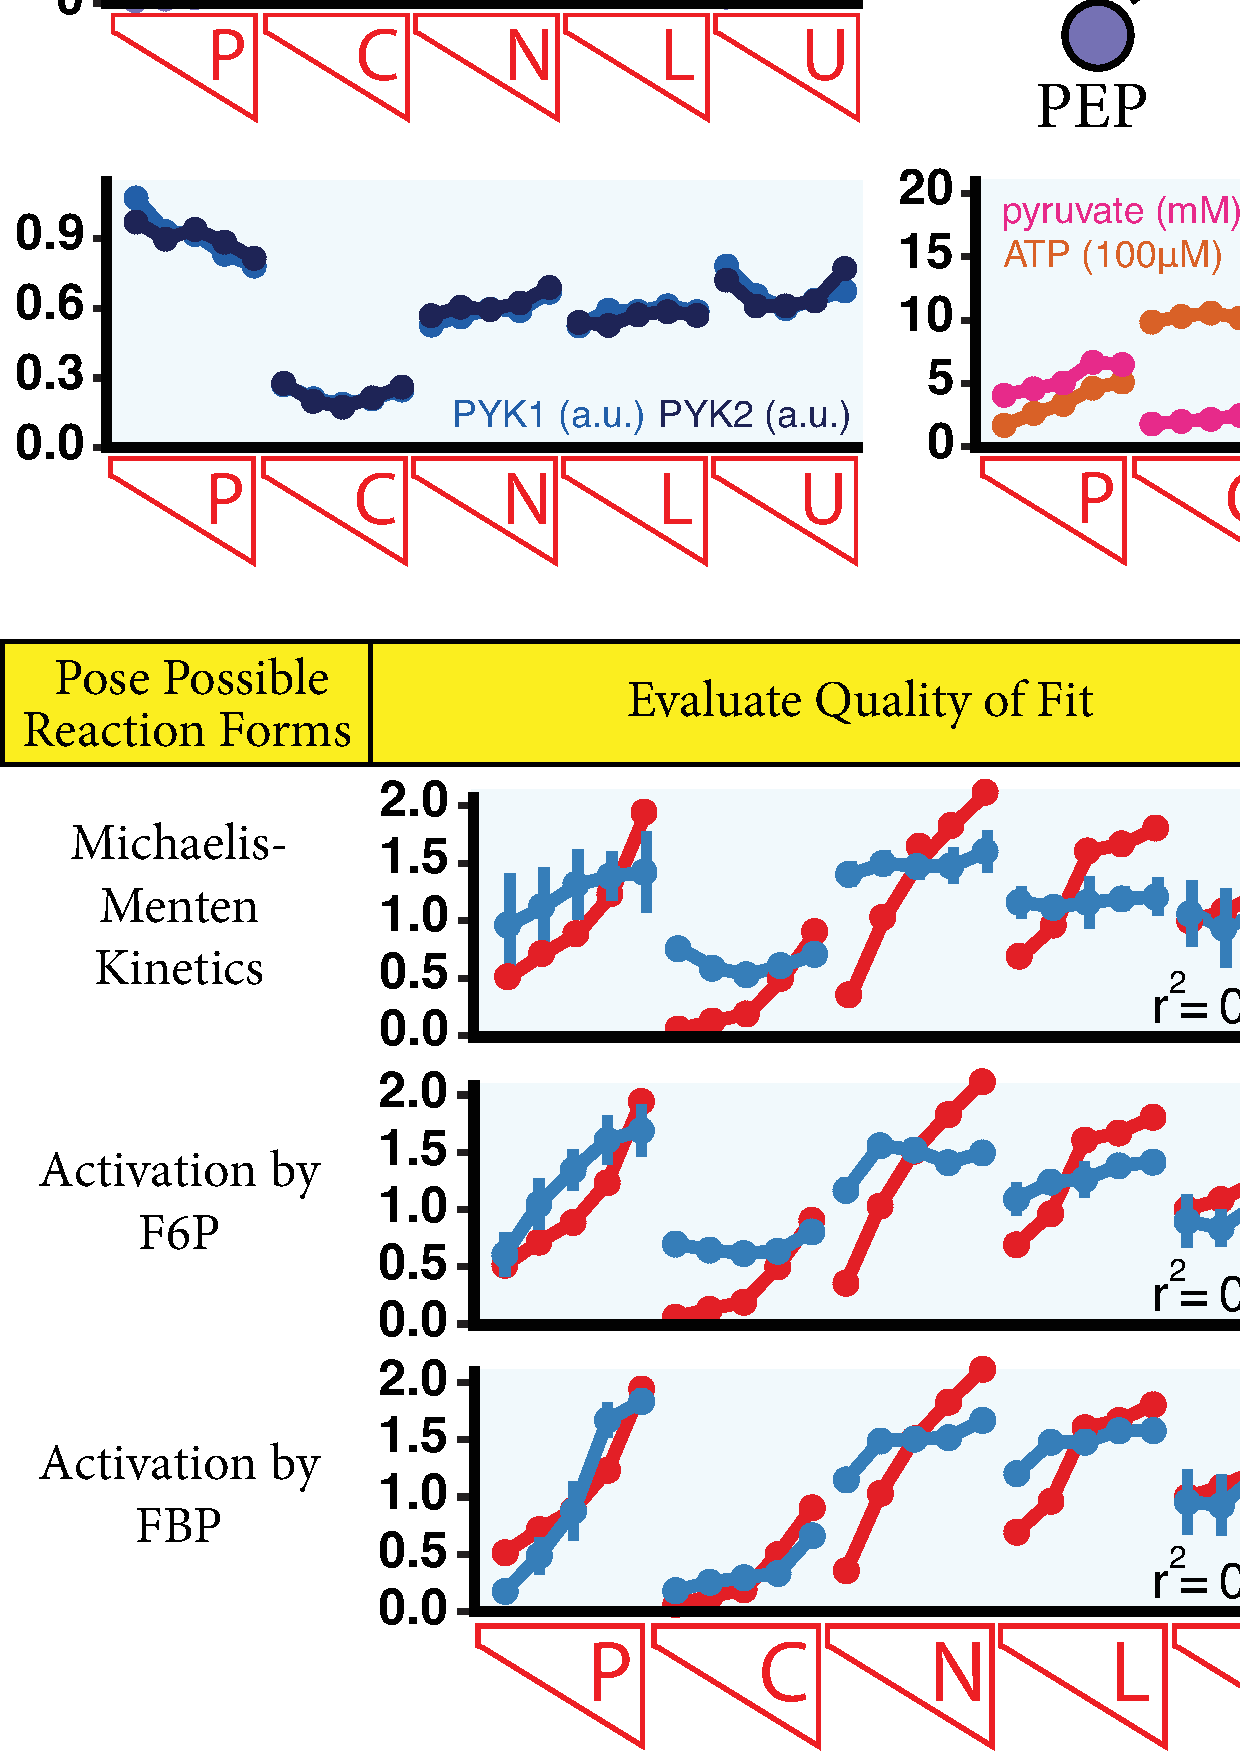
\includegraphics[width = 1\textwidth]{ch-simmer/Figures/F4-identifyingRegulation.pdf}
\caption[Two models of PRPP Amidotransferase (PPAT) kinetics are compared: reversible Michaelis-Menten kinetics with and without allosteric inhibition by AMP]{Two models of PRPP Amidotransferase (PPAT) kinetics are compared: reversible Michaelis-Menten kinetics with and without allosteric inhibition by AMP.  \textbf{A)} Across 25 conditions, we measured the relative concentrations of both substrates (PRPP:phosphoribosyl pyrophosphate and Gln:glutamine), and one product (Glu:glutamate) and the enzyme (ADE4). Unmeasured species were treated as being invariant across the measured conditions. \textbf{B)} If Michaelis-Menten kinetics is approximately true \textit{in vivo}, then measured flux should be a Michaelis-Menten function of substrates, products, and enzymes concentrations.  While Michaelis-Menten kinetics predicts the average flux through chemostats with the same limiting nutrient, it is unable to account for increasing flux with growth-rate.  \textbf{C)} Using measured concentrations of AMP (adenosine monophosphate), treating AMP as allosteric inhibitor results in a statistically-significant improvement in how well flux can be predicted relative to the simple Michaelis-Menten kinetics (p $<$ 3x10$^{-5}$, q $<$ 0.1).}
\label{fig:PPAT}
\end{figure}

\subsection{Strategy for combining systems-level data and prior knowledge to identify physiologically relevant regulators.}

In principle, the SIMMER approach can identify allosteric regulation without reliance on prior knowledge, by examining for each reaction whether inclusion of each measured metabolite as an activator or inhibitor significantly improves the fit. To test this approach, we assembled an unbiased list of gold-standard physiological allosteric metabolic regulation in yeast by comprehensively summarizing existing reviews of yeast metabolic regulation \cite{Jones:1982dn, Sekine:2007ej, Fraenkel:2011wp}. Among these instances of physiological regulation, 22 regulators of 16 reactions (Table S2) could be tested to evaluate whether SIMMER would recapitulate this regulation. In individual testing of these 22 regulators, 45\% greatly improved the fit (p $<$ 0.01). This fraction far exceeded other reported biochemical regulators of these enzymes (22\%) or randomly selected metabolites (20\%). Testing of all possible candidates, however, produced an unwieldy number of metabolites that significant enhanced fit whether biochemical regulators, or all measured metabolites were considered (average of 3.4 and 43.4 per-reaction respectively). This is not due to each of these regulators being physiologically significant, but instead reflects strong correlations between the concentrations of many metabolites, such that when one improves the fit, several other also do. Moreover, this excess of predicted regulators remains after correcting for the reaction-wise false positive rate, 

Because the quantitative influence of many metabolites cannot be distinguished, we focused on developing an approach that integrates existing literature knowledge. Some biochemical characterization had been performed for each of the 55 reactions for which we had complete integrative `omics data, including for the relevant Baker's yeast enzyme in 33 cases. This prior work, as summarized in the BRENDA database \cite{Scheer:2011df}, was used to assemble a list of putative regulators for each reaction. We sought to determine which of these candidate regulators, drawn from across any species, could be shown using SIMMER to be physiologically meaningful in yeast.
 
To integrate our data and prior literature knowledge, we took a Bayesian approach, aiming to maximize $Pr(Model | Data)$, where ``Model'' is a Michaelis-Menten equation including regulation and 
``Model'' is ``True'' if the regulation is physiologically meaningful \cite{Gelman:2003vk}. Using Bayes Theorem, 

\begin{equation}
Pr(Model | Data) = Pr(Data | Model) Pr(Model) / Pr(Data)\label{eqtn-bayes1}
\end{equation}

$Pr(Data | Model)$ can be assessed as above based on least squares deviations between measured and predicted flux (i.e. how well concentrations predict the fluxes). As $Pr(Data)$ is independent of the choice of the model, thus 

\begin{equation}
Pr(Model | Data) \propto Pr(Data | Model) Pr(Model) \label{eqtn-bayes2}
\end{equation}

To assess the \textit{a priori} probability of different models, for the 16 reactions for which we had identified gold standard regulators, we compiled a list of all known literature regulation by measured metabolites (240). We then treated the 22 instances of gold standard regulation as ``True'' models, and assessed which literature metrics might differentiate these gold standard cases. Via regression analysis, we found that the log-odds of a regulator falling in the gold standard list increased strongly with the number of regulatory annotations in BRENDA, both within yeast (p $<$ 0.002) and across non-yeast species (p $<$ 0.0002), and decreased as the total number of regulators of a reaction assessed grew (p $<$ 0.02). The resulting regression equation allows us to establish $Pr(Model)$ for any candidate regulator based on these three numerical metrics from the BRENDA database. This approach conservatively enforces that, even among putative regulators listed in BRENDA, physiologically meaningful regulation is a priori unlikely (median probability of $\sim$ 0.03), especially for well-studied reactions where the list of putative regulators is long.  


\subsection{Identification of 32 instances of physiologically meaningful yeast metabolic regulation.}

Using the above strategy, we assessed $Pr(Model | Data)$ (i.e., the probability that the regulation is physiologically significant) for each candidate literature regulator of the 56 reactions for which we had complete `omics data. For reactions where we identified one or more regulators significantly improved fit (q-value $<$ 0.1), we tested whether cooperative binding of regulators, or the inclusion of a secondary regulator further improved fit.

By balancing the inherent plausibility of each regulatory model, $Pr(Model)$, with its quantitative support, $Pr(Data | Model)$, the model which is best supported for each reaction could be found $Pr(Model | Data)$. In this manner, we identified 32 instances of physiologically relevant regulation, including five reactions with two physiological regulators and two reactions with cooperative regulation (Table S2, Figure 5). These 32 instances of regulation encompassed 5 instances of ``gold standard'' yeast regulation, YY instances of biosynthetic feedback inhibition that have been previously shown to be physiologically relevant in other organisms but not yeast, and ZZ instances of regulation that had, to our knowledge, previously been characterized only biochemically and thus was generally not considered meaningful.



%%%%%

In addition to the regulation of ADE4 by AMP, additional canonical regulators that were predicted over all alternative regulators include regulation of aspartokinase (HOM3), homocitrate synthase (LYS20/LYS21), glutamate-5-kinase (PRO1) and acetolactate synthase (ILV2,6) by threonine, lysine, proline and ATP, respectively \cite{WYNGAARDEN:1959wf, Jones:1982dn, Sekine:2007ej}

By reproducing the best supported regulation in yeast over weaker candidates, SLIMER distills \textit{in vivo} regulation when our results conform to prevailing knowledge, but the real power of this approach is that a multitude of understudied regulatory hypotheses can be efficiently evaluated and statistically compared.  To demonstrate the utility of this approach for computationally-guided discovery, we chose two well-studied reactions where predicted regulation departs from canon, and for each reaction, precise molecular hypotheses were tested using \textit{in vitro} biochemistry.  Studying ATP-phosphoribosyltransferase (ATP-PRTase; HIS1), we found that the canonical inhibition by histidine was likely insufficient, because this inhibition is strongly contingent upon ATP-PRTase's product, phosphoribosyl-ATP (Figure \ref{fig:atpprtase}).  This combinatorial regulation has previously been suggested in \textit{e. coli} but we are the first to report its relevance in \textit{S. cerevisiae} \cite{DallLarsen:1976wm}.  Investigating ornithine transcarbamylase (OTCase; ARG3), an enzyme that is not commonly thought to be regulated through allostery \cite{Jones:1982dn}, our method predicts that alanine could serve as a physiological inhibitor.  Using both spectrophotometric and mass spectrometric assays, we confirmed that alanine inhibits Arg3p with a k$_{i}$ of 15 mM (\hyperref[fig:otcase]{Figure \ref{fig:otcase}}).  Given physiological concentrations, alanine, and to a lesser extent the other aliphatic amino acids, will differentially impact OTCase flux.  One implication of this regulation is that amino acid concentrations could indirectly stimulate ribosome synthesis, possibly allowing for a metabolic coordination of amino acid abundance and ribosome synthesis.

\subsection{Global analysis.}
 
By allowing researchers to evaluate the support for alternative kinetic models that can then be interrogated through directed experiments, SLIMER is a powerful tool to study individual reactions.  The greatest benefit of this approach however, is that the same dataset can provide comparable insight into reactions distributed across metabolism.  Our data were sufficient to inform the kinetics of 56 reactions across central carbon metabolism, amino acid synthesis and nucleotide metabolism.  For each reaction, reversible Michaelis-Menten kinetics was compared to models of regulation drawn from BRENDA and for those regulatory mechanisms that significantly improved fit, significant regulatory mechanisms were augmented by either allowing for regulator cooperativity or including a second regulator. The support for each kinetic model can be summarized based on how well it conforms to the data (Pr(data$|$model)) and its plausibility (Pr(model$|$literature)).  These models can be compared, while penalizing complicated models using Akaike Information Content with Correction (AICc) \cite{Burnham:2002eq}. Through model comparison, the best supported kinetic model of each reaction was determined, while we we also noted alternative supported regulatory mechanisms for each reaction (Table S2).

Inspecting the best-fit reaction forms for each of the 56 studied reactions, the kinetics of twelve reactions could not be approximated by any tested model (spearman correlation $<$ 0.6), while the remaining 44 reactions were reasonably fit by either generalized Michaelis-Menten kinetics (16 reactions) or models including some regulation (28 reactions) (Figure 4).  For eight of these reactions, further improvement was possible through the addition of a secondary regulator, or allowing for regulator cooperativity.  Metabolite affinities implied by the reaction forms agree with literature estimates \cite{Scheer:2011df}, with substrates and products varying between unsaturated and saturated on a case-by-case basis, but regulators operating at concentrations near their affinity, where the greatest tuning of flux is possible (\hyperref[fig:occupancy]{Figure \ref{fig:occupancy}}). Inferred thermodynamics are consistent with previous estimates of free energy drops across glycolysis \cite{Flamholz:2013io}, and for near-equilibrium reactions, there is an important role for metabolite concentrations shifting the ratio of forward to reverse flux across nutrient conditions (\hyperref[fig:paramaterValues]{Figure \ref{fig:paramaterValues}}).



\begin{figure}[h!]
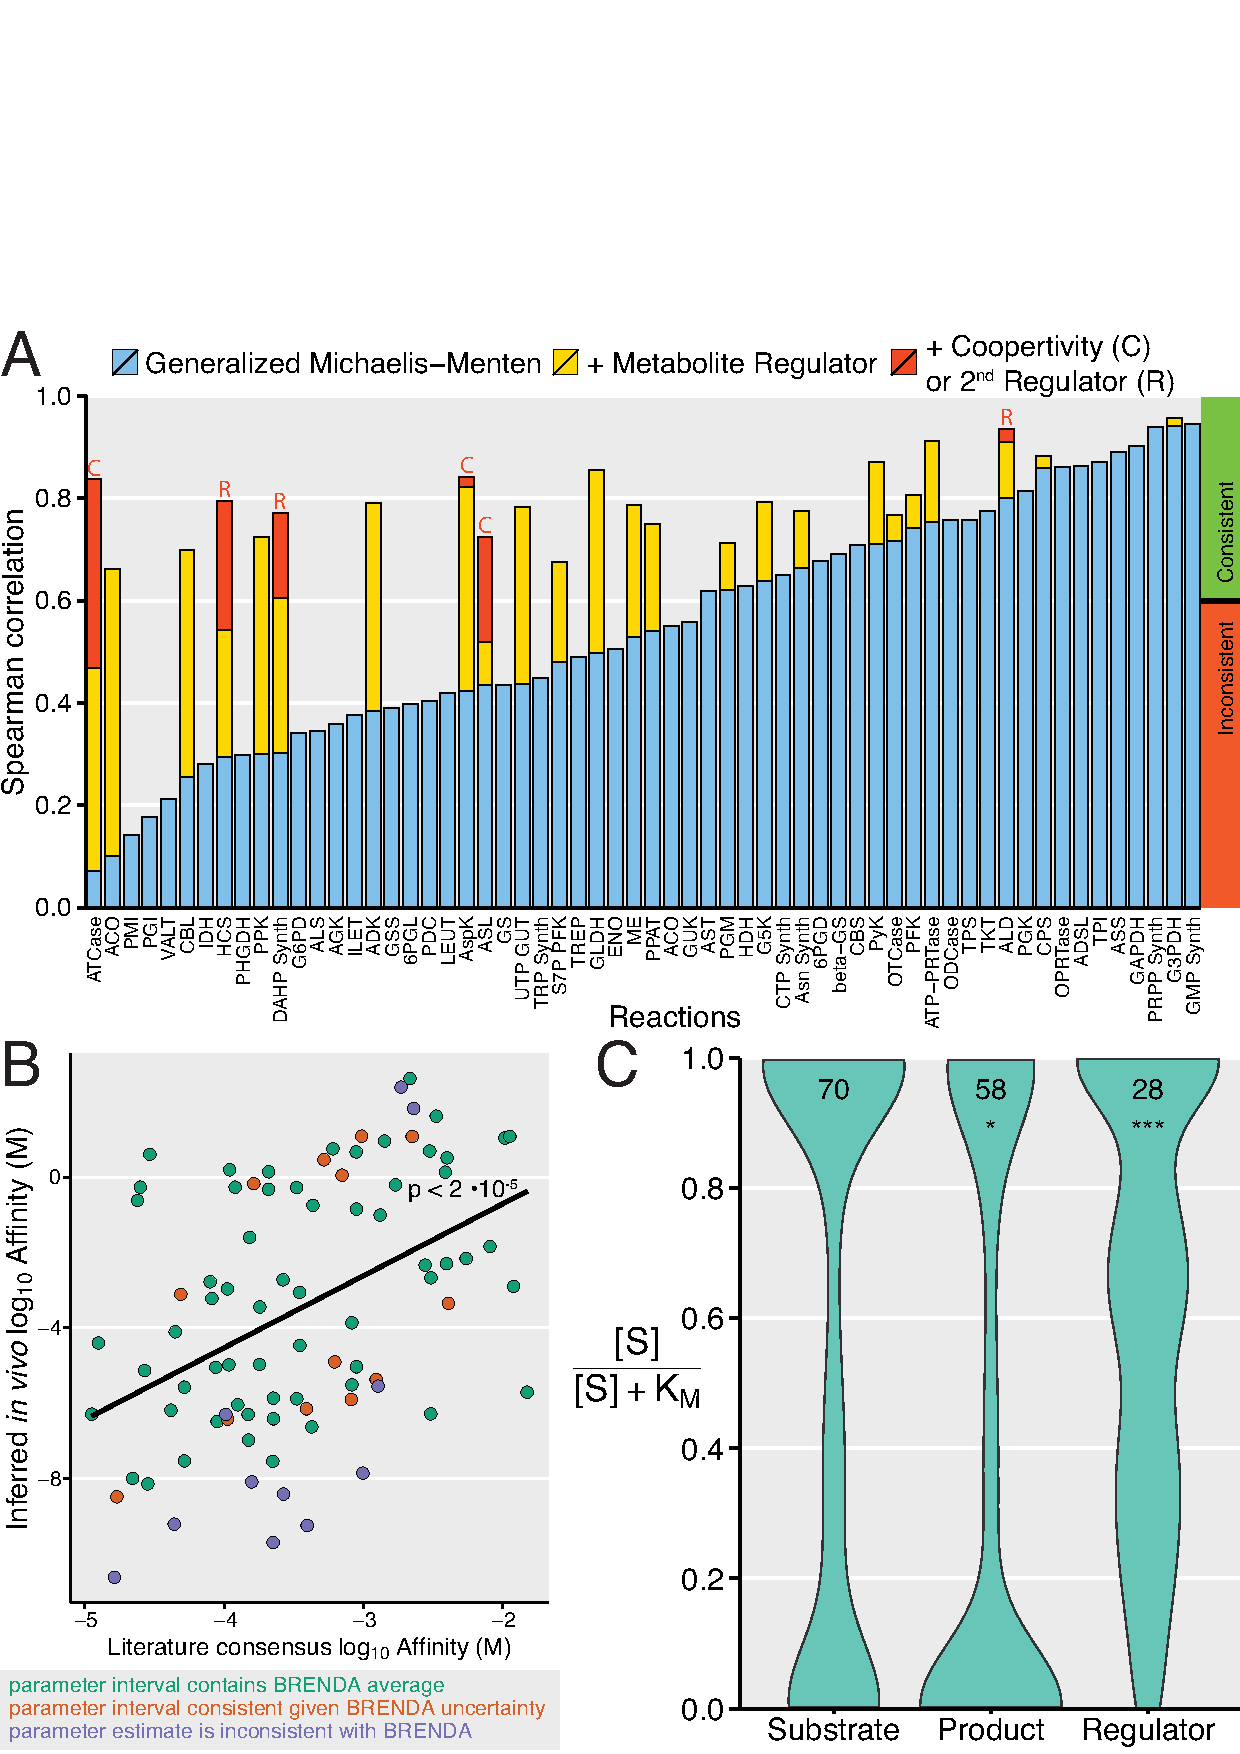
\includegraphics[width = 1\textwidth]{ch-simmer/Figures/F5-performanceSummary.pdf}
\caption[Metabolism-wide summary of the consistency between measured flux and Michaelis-Menten predictions]{Metabolism-wide summary of the consistency between measured flux and Michaelis-Menten predictions. For each of 56 reactions, the spearman correlation between measured flux and flux implied by Michaelis-Menten kinetics (with and without regulation) is shown.  For 29 reactions, inclusion of a regulator was supported, and for eight of these reactions, further improvement is possible through a secondary regulator or regulator cooperativity.  For reactions with supported regulation, the improvement in spearman correlation relative to the best-supported simpler models is shown.}
\label{fig:allosteryFit}
\end{figure}

While we are exploring a large number of possible regulators drawn from BRENDA, these candidates still represent a small fraction of possible regulatory interactions that could exist. Identifying purely novel regulation may require checking all metabolites, but this brute force method is computationally inefficient and is also statistically unsound to due to dependence between hypotheses. To deal with these challenges, we used an alternative approach to look for purely novel regulation. Because the concentrations of possible activators and inhibitors are spanned by the metabolomic principal components, we reasoned that the trend of an optimal metabolic regulator could be found by jointly optimizing the relative abundance profile of a metabolite (via principle component loads) and the kinetic effect of this regulator (via kinetic parameters). This approach was used to identify an ``optimal'' activator and inhibitor of each reaction whose relative abundance trend could then be compared to other measured metabolites, resulting in significance rankings similar to when all metabolites are separately tested (spearman correlation, 0.44; p $<$ 1 $\times 10^{-16}$). The power of this approach is limited in this study due to model complexity but can still suggest possible regulators when either no tested reaction form is quantitatively supported or few regulatory hypotheses exist (\hyperref[fig:hypoMet]{Figure \ref{fig:hypoMet}}). Using this approach, we see that reactions with no adequate reaction form could not be rescued by an optimal regulator, suggesting some greater pathology than missing regulation, while for understudied regulation, one reaction, guanylate kinase (GUK1) showed evidence of regulation.

\subsection{Assessing how metabolites and enzymes change flux.}

In order to reach a clean alignment of measured flux and a kinetic model's prediction, this model implicitly accounts for the extent of concentration variability for each reaction specie and the impact of this variation on flux.  Not all reaction species are equally important in this regard; some species may remain at nearly fixed concentration or changes in their concentration may not change flux (e.g. saturated metabolites or minor isoenzymes).  To understand which species are important in driving variable flux through each reaction, we need a quantitative way to dissect the combined role of all species in driving variable flux into the marginal contribution of each metabolite and enzyme.  A specie's role in driving variable flux is related to two factors: the magnitude by which a specie's concentration varies and the way in which flux through the reaction responds to changes in this specie's concentration.  The influence of a single specie, its \textit{metabolic leverage}, is roughly proportional to the product of its fold-change and average elasticity $\left(\epsilon = \frac{\partial F}{\partial S}\frac{[S]}{F}\right)$ \cite{Kacser:1973fe, Liao:1993in}.

Calculating metabolic leverage for each of the 44 well-fit reactions, allows us to determine how the total variable flux in these reactions has resulted from changes of reaction species.  Summarizing the relative influence of substrates, products, enzymes and regulators (\hyperref[fig:metabolicLeverage]{Figure \ref{fig:metabolicLeverage}}, \hyperref[fig:MLbar]{Figure \ref{fig:MLbar}}) - we see that reversible reactions are almost entirely driven by changes in substrate and product concentrations although the relative influence of substrates and products varies from reaction to reaction.  In contrast, irreversible reactions are driven primarily by substrate and enzyme concentrations, and for select reactions, regulators also have an important role. In the vast majority of cases, even when strong regulation exists, a single regulator rarely dominates, instead, flux is collectively dictated by substrates, enzymes and regulators.

\begin{figure}[H]
\floatbox[{\capbeside\thisfloatsetup{capbesideposition={right,top},capbesidewidth=6cm}}]{figure}[\FBwidth]
{\caption[Flux change in response to changing concentrations of metabolites and enzymes whose impact on flux is governed by the metabolites' and enzyme's elasticity]{\fixedspaceword{Flux change in response to changing concentrations of metabolites and enzymes whose impact on flux is governed by the metabolites' and enzyme's elasticity.  The impact of a single metabolite or enzyme in driving variable flux is roughly proportional to its elasticity weighted by the standard deviation of log relative concentrations across physiological conditions (phosphate, carbon and nitrogen limitations).  For a reaction, the relative contributions of its enzymes, substrates and regulators in driving variable flux across physiological conditions can be approximated by this metabolic leverage.  \textbf{A)} Metabolic leverage can be projected onto a ternary surface where each reaction is effected by enzymes, substrates, products, and possibly regulators whose influence sums to 100\% leverage.  \textbf{B)} This metric is able to distinguish reactions that are irreversible and thus likely to be good points of regulation from more passive reversible reactions. Reactions are classified as kinetically irreversible if literature suggests that net flux only proceeds in the forward direction \cite{Heavner:2012dg}. \textbf{C)} Pie chart summary of average metabolic leverage for irreversible and reversible reactions.
}}\label{fig:metabolicLeverage}}
{\includegraphics[width=\textwidth-6cm]{ch-simmer/Figures/F6-MetabolicLeverage.pdf}}
\end{figure}


When reactions respond strongly to changes in enzyme or regulator concentrations, it is likely that these regulatory events causally change flux or metabolite concentrations.  We can test this assertion, which links metabolic leverage to metabolic control, by studying glycolysis where reaction kinetics are well-fit, allowing a comparison of reaction-level and pathway-level inference.  Using the optimal reaction forms for glycolytic reactions, two metabolic control analysis (MCA) models of glycolysis were created which contrast the metabolic consequences of two similarly supported regulatory mechanisms for pyruvate kinase \cite{Cortassa:1994is, Westerhoff:1987jo}. This model reproduces the finding that glycolytic flux is predominately governed by phosphofructokinase (PFK; PFK1,2) \cite{Cortassa:1994is}, while the feed-forward regulation on pyruvate kinase (PyK; CDC19, PYK2) by fructose 1,6-bisphosphate primarily changes metabolite concentrations rather than flux per-se in line with experimental findings \cite{Xu:2012gg} (\hyperref[fig:MCA]{Figure \ref{fig:MCA}}). Projecting metabolic leverage onto a metabolic map (\hyperref[fig:MLpathways]{Figure \ref{fig:MLpathways}}), it is clear that phosphofructokinase and pyruvate kinase are the most important regulatory reactions in glycolysis.  This agreement suggests that metabolic leverage can provide a first-glance at the control of pathways (\hyperref[fig:MLpathways]{Figure \ref{fig:MLpathways}}) when comprehensive analysis using MCA is not immediately possible.  For instance, production of structural glucans is governed by the concentration of the beta-glucan synthases (FKS1, GSC2), while the production of aspartate family amino acids, as well as the interconversion of purines and pyrimidines operates without external regulation; instead, flux is driven solely by changes in substrate and product concentrations. 

\section{Discussion}

As we move from understanding the behavior of individual metabolic pathways to understanding metabolism as a complete system, there is a pressing need for methods that excel at these larger scales. Previous attempts to infer metabolic regulation have evaluated model support at a systems-level.  This has forced researchers either to use strong \textit{a priori} assumptions about how metabolism functions (and thereby only explore a small amount of hypothesis space) \cite{Chassagnole:2002ty, Zampar:2013fr} or to restrict their focus to relatively small metabolic networks that could be comprehensively interrogated \cite{Link:2013dj}, albeit with poor scaling ($\mathcal{O}(n^{m})$ for $n$ reactions and $m$ possible reactions forms of each reaction. By measuring flux, rather than inferring it based on changing metabolite concentrations, reactions can be rendered independent, and metabolism can be studied on a reaction-by-reaction basis. When this approach is adopted, metabolic inference scales linearly with the number of reactions and the number of regulators we want to consider for each reaction ($\mathcal{O}(nm)$). Furthermore, each reaction-level model can be evaluated more quickly than metabolism-level models, and correct models of individual reactions can be found without necessitating that the kinetics of all reactions be correct. In our study, we used this approach to push beyond pathway-level analysis to investigate metabolic regulation at the level of complete metabolism. We used this approach to address two outstanding challenges in chemical biology: how to systematically identify physiological regulation that may be entirely novel and whether `omic data can elucidate the physiological control of flux.

These topics are extremely important in microbial metabolic engineering, where researchers frequently attempt to preferentially direct flux through pathways of interest.  Because microbial metabolism has evolved chiefly to exhibit robustness, native regulation ingrained in the metabolic network is frequently at odds with design goals \cite{Kitano:2007cp}.  As such, pathway engineering efforts are frequently hampered when cryptic metabolic regulation exists or the relationship between pathway fluxes and enzyme abundance is unclear.  Using SLIMER, solutions to both challenges can be found.  When a native allosteric regulator is important, this regulation can be identified based on its physiological impact, allowing targeted experiments to abolish the regulators binding. To determine how enzyme levels should be tweaked to alter pathway flux, we hypothesize that for select reactions where flux strongly tracks enzyme abundance, by mimicking physiological control mechanisms, over-expressing enzymes will result in changes in flux.  Our analysis suggests that such examples are rare, paralleling experimental observations that pathway fluxes are rarely limited by the expression of a single enzyme \cite{Hauf:2000vu, CornishBowden:1995fy}.  For such pathways where flux dependents upon multiple reactions, we have demonstrated, using glycolysis as an example, that the physiological reaction forms which we have inferred can be coupled together to provide a more accurate characterization of pathway control.

In this study, we have focused on characterizing the metabolism of \textit{S. cerevisiae}, a microbe whose metabolism is relatively well understood, but our approach can be applied to any organism that can be grown in suspension where metabolic behavior can be varied using either nutritional or genetic perturbations.  We feel that this approach will be particularly useful for providing a preliminary understanding of lesser understood organisms, where traditional approaches based on studying one enzyme at a time, are intractable.  Beyond providing such a one-shot characterization of metabolism, most lesser understudied organisms will contain reactions which have been scarcely biochemically characterized.  We have provided solutions for identifying regulation using little prior literature knowledge by either capitalizing upon regulatory conservation or searching for purely novel regulation by an optimum regulator.

While our data is the most comprehensive enzyme-metabolite-flux dataset to date, it is still not a complete collection of all relevant metabolic information.  To fulfill the promise of SLIMER will require both progressively refining our input data and and expanding the breadth of our analysis.  Improving our current data will largely depend upon improving the number of distinct metabolites that can be measured through metabolomics and improving the accuracy of flux determination.  Here, advances in instrumentation paired with more focused analytical methods should afford both a more accurate and comprehensive detection of relevant metabolites, and the use of stable isotope labeling could further improve flux accuracy \cite{Yuan:2008er}.  Expanding the breadth of our dataset will entail addressing biological phenomena that were beyond the scope of this study.  Chiefly, we are unable to assess the extent to which flux is impacted by post-translational regulation \cite{Fiedler:2009hx, Schulz:2014eo}, variable sub-cellular localization \cite{Kitamoto:1988wc} or cell-to-cell variability \cite{Tu:2005cv}.  These limitations are likely to blame for the 12 reactions where no adequate kinetic model could be found, although inaccurate measurements or missing regulation could also result in inappropriate regulatory predictions that partially compensate for unmeasured factors.  A final issue of note is that we had to make assumptions about the form of rate laws, and while true \textit{in vivo} rate laws rarely reduce to generalized Michaelis-Menten kinetics \cite{Hill:1977vm}, our reaction forms are able to achieve an approximately correct relationship between species and resulting flux across the physiological conditions investigated and thus these simplified kinetics are functionally sufficient for our purposes \cite{Fell:1997wg}.

Because we have characterized a reproducible set of conditions that contain much of the meaningful metabolic variation in yeast, we hope that this study will serve as an important scaffold for future work to build upon, whether by incorporating additional experimental information on existing conditions or by expanding the breadth of the study by characterizing additional conditions. Regulation can only be identified if it differentially impacts study conditions. By expanding the number of conditions that are investigated, we can unmask regulation that is important in these conditions, and our approach can identify this regulation by virtue of the kinetic importance it gains in these new conditions. This will also serve to refine the accuracy of parameter estimates from reaction forms and better discriminate  competing regulatory hypotheses.

\section{Supplemental Figures and Tables}

\setcounter{figure}{0}
\makeatletter 
\renewcommand{\thefigure}{\thechapter.S\@arabic\c@figure}
\renewcommand{\thetable}{\thechapter.S\@arabic\c@table}
\makeatother



\begin{figure}[H]
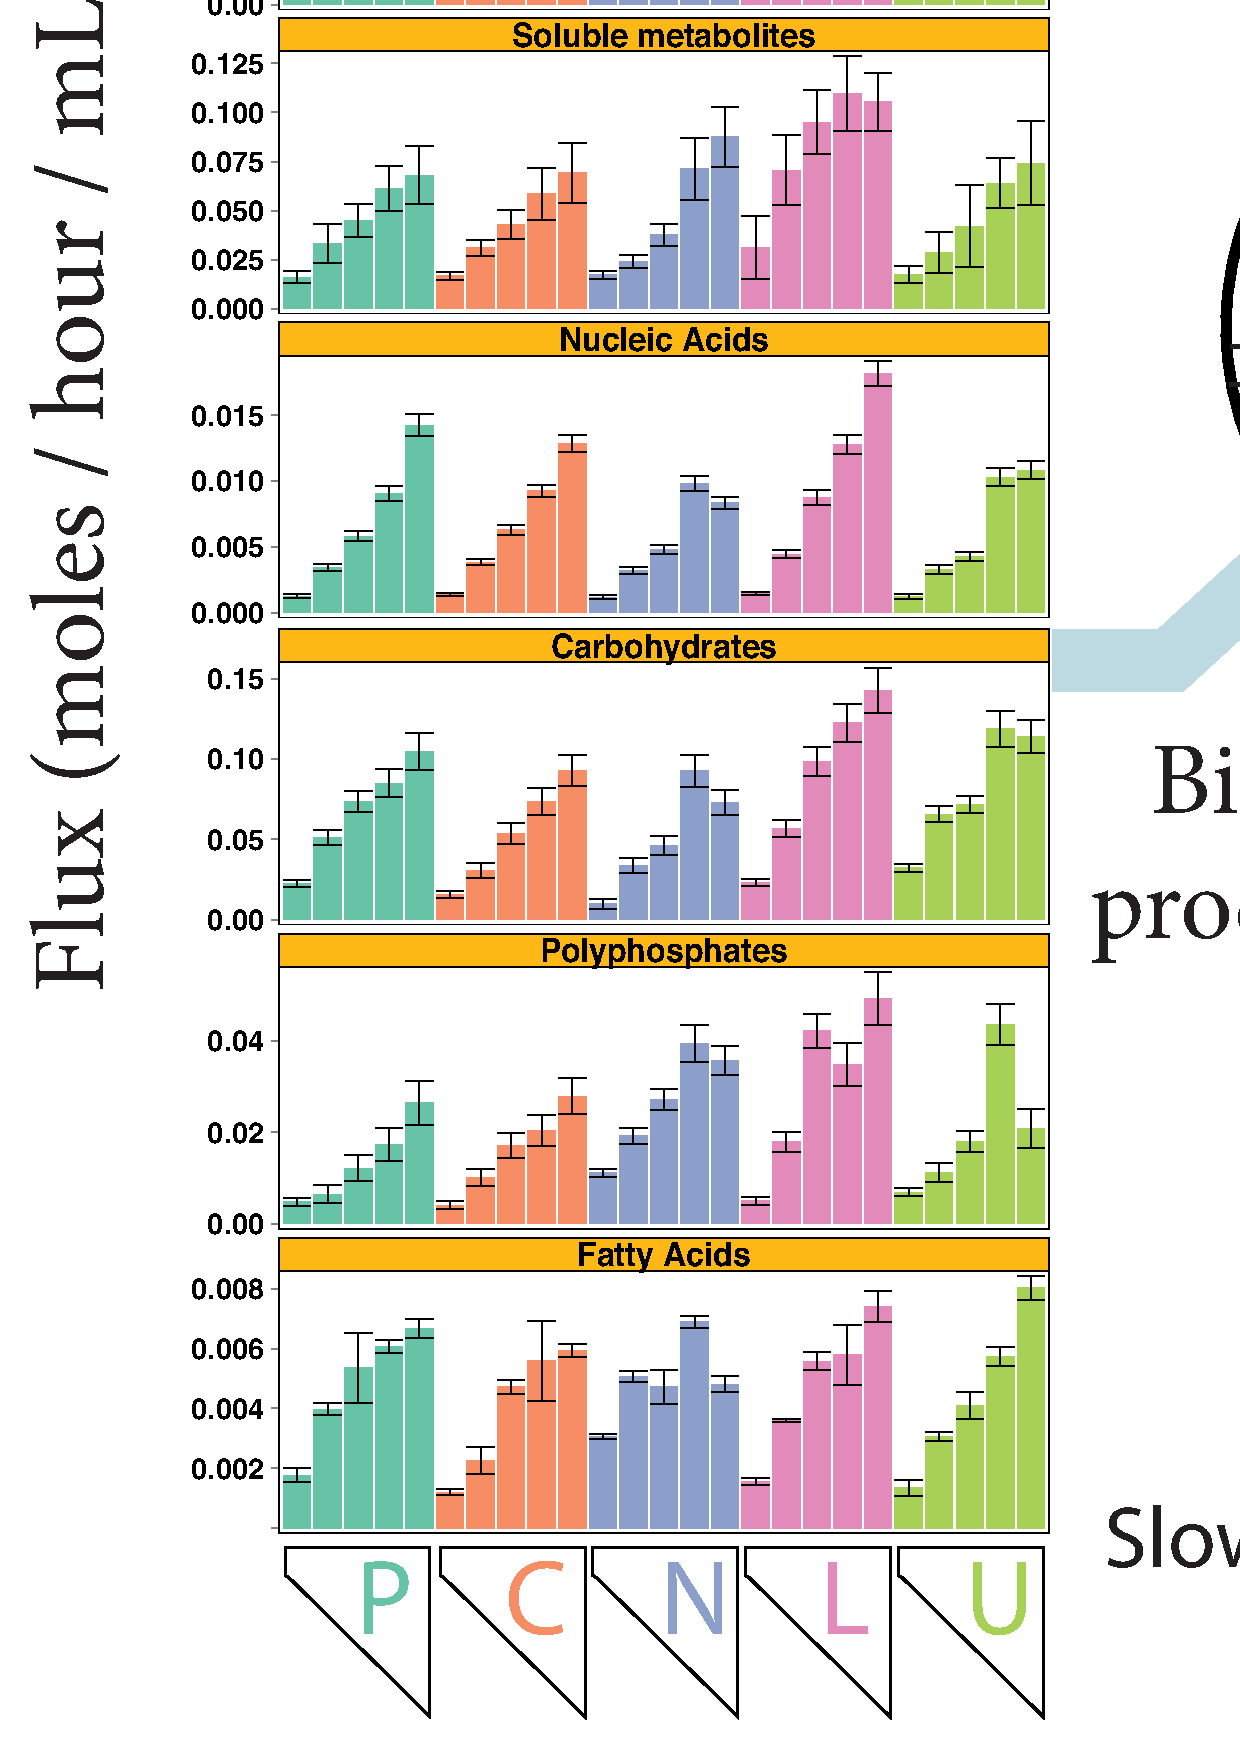
\includegraphics[width = 0.8\textwidth]{ch-simmer/Figures/Supplement/boundaryFluxes.pdf}
\caption[Summary of experimentally-determined rates of metabolite uptake, excretion and incorporation into biomass for each chemostat condition]{Summary of experimentally-determined rates of metabolite uptake, excretion and incorporation into biomass for each chemostat condition.}
\label{fig:boundFlux}
\end{figure}

\begin{figure}[H]
\includegraphics[width = 0.7\textwidth]{ch-simmer/Figures/Supplement/fluxHM.pdf}
\caption[Heatmap summarizing relative flux through 233 reactions across chemostat conditions]{Heatmap summarizing relative flux through 233 reactions across chemostat conditions.  Absolute reactions fluxes were determined independently for each chemostat and to visualize reactions whose flux was correlated, the flux through each reaction was expressed relative to the median absolute flux across all conditions.  Reactions were organized using hierarchical clustering using absolute pearson correlation with average linkage.  Only reactions that were well-constrained based on flux variability analysis are shown.}
\label{fig:fluxHM}
\end{figure}

\begin{figure}[H]
\includegraphics[width = 0.5\textwidth]{ch-simmer/Figures/Supplement/peptide_RA_reproduce.pdf}
\caption[Nutrient-induced changes in peptide abundance between technical replicates are highly reproducible]{Nutrient-induced changes in peptide abundance between technical replicates are highly reproducible.  As a representative example, a slow growth nitrogen-limited chemostat (n0.05) is compared to an internal reference slow-growth phosphorous-limited $^{15}$N-labelled chemostat ($^{15}N$-p0.05).  For each of two technical replicates, derived from independent digestion, fractionation and mass spectrometry of a single sample, the relative abundance of unlabelled experimental peptides relative to $^{15}N$-labelled reference peptides is shown.}
\label{fig:proteomicsConsistency}
\end{figure}

\begin{figure}[H]
\includegraphics[width = 0.7\textwidth]{ch-simmer/Figures/Supplement/proteinHM.pdf}
\caption[Heatmap summarizing the variable concentration of 1187 proteins across chemostat conditions]{Heatmap summarizing the variable concentration of 1187 proteins across chemostat conditions. From the ratio of unlabelled sample peptides to matching $^{15}N$-labelled reference peptides, the abundance of each enzyme relative to a common reference was determined.  Across the 25 conditions, protein relative abundances were mean-centered, log-transformed and organized by hierarchical clustering using pearson correlation with average linkage.}
\label{fig:proteinHM}
\end{figure}

\newcommand{\multilineR}[1]{\begin{tabular}[b]{@{}r@{}}#1\end{tabular}}
\newcommand{\multilineL}[1]{\begin{tabular}[b]{@{}l@{}}#1\end{tabular}}
\newcommand{\multilineC}[1]{\begin{tabular}[b]{@{}c@{}}#1\end{tabular}}

\newcolumntype{L}[1]{>{\raggedright\let\newline\\\arraybackslash\hspace{0pt}}m{#1}}
\newcolumntype{C}[1]{>{\centering\let\newline\\\arraybackslash\hspace{0pt}}m{#1}}
\newcolumntype{R}[1]{>{\raggedleft\let\newline\\\arraybackslash\hspace{0pt}}m{#1}}

\begin{table}[H]
\centering
\begin{tabular}{l>{\hfill}p{0.5in}>{\hfill}p{0.5in}>{\hfill}p{0.5in}>{\hfill}p{0.5in}>{\hfill}p{0.5in}>{\hfill}p{0.5in}}
 \begin{sideways} \begin{turn}{-90}\textbf{Pathway}\end{turn} \end{sideways} & \begin{sideways} \multilineL{Reactions with\\measured enzymes} \end{sideways} & \begin{sideways} \multilineL{Total pathway\\reactions} \end{sideways} & \begin{sideways} \multilineL{Fraction of reactions\\with measured enzymes} \end{sideways} & \begin{sideways} \multilineL{Measured enzymes} \end{sideways} & \begin{sideways} \multilineL{Total enzymes} \end{sideways} & \begin{sideways} \multilineL{Fraction of\\measured enzymes} \end{sideways} \\ 
  \hline
\multicolumn{1}{l||}{Glycolysis / Gluconeogenesis} &  16 &  16 & 100\% &  17 &  18 & 94\% \\ 
  \multicolumn{1}{l||}{Citrate cycle (TCA cycle)} &  12 &  12 & 100\% &  12 &  12 & 100\% \\ 
  \multicolumn{1}{l||}{Biosynthesis of amino acids} &  73 &  83 & 88\% &  63 &  75 & 84\% \\ 
  \multicolumn{1}{l||}{Purine metabolism} &  37 &  52 & 71\% &  28 &  41 & 68\% \\ 
  \multicolumn{1}{l||}{Pyrimidine metabolism} &  27 &  39 & 69\% &  22 &  31 & 71\% \\ 
  \multicolumn{1}{l||}{All reactions} & 346 & 524 & 66\% & 304 & 510 & 60\% \\ 
   \hline
\end{tabular}
\caption[For major metabolic pathways, the coverage of enzymes measured through proteomics is summarized]{For major metabolic pathways, the coverage of enzymes measured through proteomics is summarized.  For each pathway, we show both the the fraction of reactions where at least one enzyme was measured, as well as the total fraction of enzymes measured.  Pathway annotation are based on KEGG.}
\label{protTable}
\end{table}

\begin{table}[H]
\centering
\begin{tabular}{|l|l|l|}
\hline
Reaction Name & Regulation & Support \\\Xhline{2\arrayrulewidth} 
3-phosphoglycerate dehydrogenase & (-) Serine & \textcolor{BurntOrange}{Alternative regulation supported}\\\hline
\multirow{2}{*}{Acetolactate synthase} & (+) ATP & \textcolor{ForestGreen}{Strongest support}\\ 
  & (-) Valine & Other GS supported\\\hline
 Acetylglutamate kinase & (-) Arginine & \textcolor{BurntOrange}{No tested model is adequate}\\\hline 
 Asparagine synthetase & (-) Asparagine & \textcolor{Cerulean}{No physiological regulation}\\\hline 
 Aspartate carbamoyltransferase & (-) UTP & \textcolor{BurntOrange}{Alternative regulation supported}\\\hline 
 \multirow{2}{*}{Aspartokinase} & (-) Homoserine & \textcolor{LimeGreen}{Supported}\\ 
  & (-) Threonine & \textcolor{ForestGreen}{Strongest support}\\\hline 
 ATP phosphoribosyltransferase & (-) Histidine & \textcolor{LimeGreen}{Supported}\\\hline 
 Carbamoyl phosphate synthase & (-) UTP & \textcolor{Cerulean}{No physiological regulation}\\\hline 
 CTP synthase & (-) CTP & \textcolor{BurntOrange}{No tested model is adequate}\\\hline 
 \multirow{2}{*}{DAHP synthase} & (-) Phenylalanine & \textcolor{LimeGreen}{Supported}\\ 
  & (-) Tyrosine & \textcolor{LimeGreen}{Supported}\\\hline 
 Glutamate 5-kinase & (-) Proline & \textcolor{ForestGreen}{Strongest support}\\\hline 
 Homocitrate synthase & (-) Lysine & \textcolor{ForestGreen}{Strongest support}\\\hline 
 Homoserine kinase & (-) Threonine & \textcolor{BurntOrange}{No tested model is adequate}\\\hline 
 \multirow{3}{*}{Phosphofructokinase} & (+) AMP & \textcolor{BurntOrange}{Alternative regulation supported}\\ 
  & (-) ATP & \textcolor{BurntOrange}{Alternative regulation supported}\\ 
  & (+) Fructose 2,6-P$_{2}$ & Not measured\\\hline 
 PRPP amidotransferase & (-) AMP & \textcolor{ForestGreen}{Strongest support}\\\hline 
 \multirow{4}{*}{Pyruvate kinase} & (-) ATP & Other GS supported\\ 
 & (+) Ammonia & Not measured\\ 
 & (-) Citrate & \textcolor{LimeGreen}{Supported}\\ 
 & (+) Fructose 1,6-P$_{2}$ & \textcolor{LimeGreen}{Supported}\\ 
   \hline
\end{tabular}
\caption[Gold-standard yeast metabolic regulation]{Gold-standard yeast metabolic regulation.  Previous analysis of 16 reactions in yeast has strongly implicated a role for 24 catalytically important regulators.  22 of these 24 regulatory relationships could be tested using the SLIMER methodology. \textcolor{ForestGreen}{Strongest support}, indicates gold standard regulation that was predicted as the best candidate physiological regulator. \textcolor{LimeGreen}{Supported}, indicates regulator's which improved fit, but were not as strongly supported as alternative literature hypotheses. \textcolor{Cerulean}{No physiological regulation}, indicates that Michaelis-Menten kinetics was supported over all literature candidates. \textcolor{BurntOrange}{Alternative regulation supported}, indicates that the tested mechanism did not meaningfully improve Michaelis-Menten kinetics, but alternative literature hypotheses were supported. \textcolor{BurntOrange}{No tested model is adequate}, indicates that among all tested regulators, none were supported.}
\label{tab:GS}
\end{table}



\begin{figure}[H]
\includegraphics[width = 1\textwidth]{ch-simmer/Figures/Supplement/HIStimecourse.pdf}
\caption[Inhibition of His1p by histidine is contingent upon the reaction product, phosphoribosyl-ATP]{Inhibition of His1p by histidine is contingent upon the reaction product, phosphoribosyl-ATP.   \textbf{A)} Cumulative flux through HIS1 shows that while reaction rate is initially independent of histidine concentration, as the reaction proceeds the effect of histidine emerges. The cumulative flux at each concentration of hisitidine can be well-explained using a cubic polynomial fit using regression. \textbf{B)} Instantaneous flux, i.e. the derivative of the fitted cumulative flux, was compared to phosphoribosyl-ATP concentration.  Flux decreases as phosphoribosyl-ATP accumulates and the inhibitory effect of histidine increases with phosphoribosyl-ATP concentrations.}
\label{fig:atpprtase}
\end{figure}

\begin{figure}[H]
\includegraphics[width = 1\textwidth]{ch-simmer/Figures/Supplement/OTCaseAla.pdf}
\caption[Alanine is a physiological regulator of ornithine carbamoyltransferase]{Alanine is a physiological regulator of ornithine carbamoyltransferase.  \textbf{A)} \textit{In vitro} measurement of the impact of alanine concentration on purified Arg3p indicates that alanine is an allosteric inhibitor with a k$_{i}$ of about 14.8 mM.  \textbf{B)} Physiological concentrations of alanine vary greatly and are around the affinity for Arg3p implying meaningful difference in occupancy and inhibition.  \textbf{C)} Alanine inhibition of OTCase could serve as a way of directing flux into pyrimidine synthesis under high-amino acid conditions that should favor ribosome production.  When pyrimidine needs are met, a paired regulation of ATCase favors flux into Arginine production for nitrogen and carbon storage.}
\label{fig:otcase}
\end{figure}


\begin{figure}[H]
\includegraphics[width = 0.6\textwidth]{ch-simmer/Figures/Supplement/hypoMetAnalysis.pdf}
\caption[Using optimal regulators to investigate the regulation of understudied reactions]{Using optimal regulators to investigate the regulation of understudied reactions.  Looking at 10 reactions which each had less than five annotated regulators, we identified both an optimal hypothetical metabolite activator and an inhibitor that resulted in the greatest improvement in fit.  \textbf{A)} Of these 10 reactions, the kinetic fit of four reactions was improved by either an optimal activator or inhibitor relative to Michaelis-Menten kinetics and three of these reactions were significant relative to models containing regulation.  \textbf{B)} For each of the three reactions were an optimal activator or inhibitor was best supported, the metabolites that are most strongly correlated with the optimal regulator were noted as regulatory candidates.}
\label{fig:hypoMet}
\end{figure}

%\begin{table}[h!]
%Excel file summarizing all supported regulation for each reaction
%\end{table}


\footnotesize
\begin{landscape}
\begin{longtable}{|L{4cm} | L{7cm} || R{1.5cm} | L{7cm} | R{1.75cm}|}
\caption[Best fitting reaction form for 45 reactions]{Best fitting reaction form for 45 reactions.}
\label{tab:all_rxn}
\hline
Reaction Name&Best Supported Regulation&Spearman Correlation&All Supported Regulation&\# Regulators Tested\\\Xhline{2\arrayrulewidth} 
1,3-beta-glucan synthase&Reversible michaelis-menten &0.69&&8\\\hline
3-deoxy-D-arabino-heptulosonate 7-phosphate synthetase&noncompetitive inhibition by keto-phenylpyruvate + noncompetitive inhibition by phosphoenolpyruvate&0.78&[phosphoenolpyruvate - AND (keto-phenylpyruvate - / L-tyrosine - / D-erythrose 4-phosphate - / L-phenylalanine -)] OR (keto-phenylpyruvate - / L-tyrosine - / D-erythrose 4-phosphate - / L-phenylalanine -)&11\\\hline
acetolactate synthase&mm activation by ATP (zero flux / overflow conditions removed) *&0.795&ATP +&6\\\hline
adenylate kinase&noncompetitive inhibition by AMP + mm activation by L-threonine *&0.91&[(L-threonine + / phosphoenolpyruvate - / L-histidine +) AND (AMP - / dATP +)] OR (AMP - / dATP +)&18\\\hline
alpha,alpha-trehalose-phosphate synthase (UDP-forming)&uncompetitive inhibition by phosphate *&0.61&phosphate -&4\\\hline
argininosuccinate lyase&Reversible michaelis-menten &0.65&&9\\\hline
argininosuccinate synthase&Reversible michaelis-menten &0.84&&3\\\hline
asparagine synthase (glutamine-hydrolysing)&Reversible michaelis-menten&0.67&&5\\\hline
aspartate carbamoyltransferase&mm activation by UTP&0.75&(UTP + / ATP +)&33\\\hline
aspartate kinase&uncompetitive inhibition (variable hill) by L-threonine &0.84&(L-lysine - / L-homoserine -) OR L-threonine -&18\\\hline
aspartate transaminase&Reversible michaelis-menten &0.62&&12\\\hline
ATP phosphoribosyltransferase&uncompetitive inhibition by AMP &0.91&AMP - OR L-histidine -&4\\\hline
carbamoyl-phosphate synthase (glutamine-hydrolysing)&Reversible michaelis-menten &0.86&&33\\\hline
citrate to cis-aconitate(3-)&uncompetitive inhibition by isocitrate &0.65&isocitrate -&9\\\hline
cystathionine beta-synthase&mm activation by S-adenosyl-L-methionine &0.80&S-adenosyl-L-methionine +&5\\\hline
cystathionine g-lyase&noncompetitive inhibition by L-alanine &0.70&L-alanine -&6\\\hline
fructose-bisphosphate aldolase&noncompetitive inhibition by AMP &0.90&AMP - OR ADP -&31\\\hline
glucose 6-phosphate dehydrogenase&noncompetitive inhibition by phosphoenolpyruvate + noncompetitive inhibition by AMP &0.73&[phosphoenolpyruvate - AND AMP -] OR AMP -&14\\\hline
glutamate 5-kinase&uncompetitive inhibition by L-proline &0.79&L-proline -&4\\\hline
glutamate dehydrogenase (NADP)&uncompetitive inhibition (variable hill) by quinolinate &0.89&quinolinate -&49\\\hline
glyceraldehyde-3-phosphate dehydrogenase&Reversible michaelis-menten &0.90&&19\\\hline
glycerol-3-phosphate dehydrogenase (NAD)&Reversible michaelis-menten &0.94&&15\\\hline
GMP synthase&Reversible michaelis-menten &0.94&&3\\\hline
guanylate kinase&noncompetitive inhibition by GMP &0.68&GMP -&3\\\hline
histidinol dehydrogenase&Reversible michaelis-menten &0.64&&0\\\hline
homocitrate synthase&noncompetitive inhibition by quinolinate + uncompetitive inhibition by L-lysine &0.79&[(L-lysine - / L-arginine -) AND (quinolinate - OR dATP +)] OR (L-lysine - / L-arginine -) OR dATP +&9\\\hline
malic enzyme (NAD)&noncompetitive inhibition by AMP &0.79&AMP -&32\\\hline
ornithine carbamoyltransferase&competitive inhibition by L-alanine &0.76&L-alanine -&27\\\hline
orotate phosphoribosyltransferase&Reversible michaelis-menten &0.86&&16\\\hline
orotidine-5'-phosphate decarboxylase&Reversible michaelis-menten &0.76&&16\\\hline
phosphofructokinase&noncompetitive inhibition by AMP &0.85&AMP - OR D-fructose 1,6-bisphosphate + OR isocitrate -&27\\\hline
phosphofructokinase (s7p)&noncompetitive inhibition by phosphoenolpyruvate &0.67&phosphoenolpyruvate - OR AMP -&27\\\hline
phosphogluconate dehydrogenase&mm activation by L-aspartate &0.77&L-aspartate +&18\\\hline
phosphoglycerate dehydrogenase&mm activation by L-methionine &0.77&L-methionine +&10\\\hline
phosphoglycerate kinase&Reversible michaelis-menten &0.81&&9\\\hline
phosphoglycerate mutase&noncompetitive inhibition by 3-phosphoglycerate &0.71&3-phosphoglycerate -&4\\\hline
phosphoribosylpyrophosphate amidotransferase&noncompetitive inhibition by AMP &0.75&AMP -&9\\\hline
phosphoribosylpyrophosphate synthetase&Reversible michaelis-menten &0.94&&20\\\hline
pyruvate decarboxylase&noncompetitive inhibition by keto-phenylpyruvate &0.78&keto-phenylpyruvate -&4\\\hline
pyruvate kinase&noncompetitive inhibition by isocitrate + noncompetitive inhibition by AMP &0.98&[(isocitrate - / citrate -) AND (AMP - OR (dihydroxyacetone phosphate + / ribose-5-phosphate + / glyceraldehyde 3-phosphate + / D-fructose 1,6-bisphosphate + / D-fructose 6-phosphate + / D-glucose 6-phosphate + / D-glucose 1-phosphate +) OR (L-alanine - / L-phenylalanine - / L-tyrosine -) OR L-glutamate - OR 2-oxoglutarate -)] OR [(L-alanine + / L-aspartate + / L-glutamine +) AND (AMP - OR 2-oxoglutarate - OR L-glutamate -)]&44\\\hline
transketolase 1&Reversible michaelis-menten &0.77&&3\\\hline
trehalose-phosphatase&mm activation by D-fructose 6-phosphate + mm activation by trehalose &0.88&[D-fructose 6-phosphate + AND trehalose +] OR D-fructose 6-phosphate +&7\\\hline
triose-phosphate isomerase&Reversible michaelis-menten (default) &0.87&&5\\\hline
UTP-glucose-1-phosphate uridylyltransferase&noncompetitive inhibition by UDP-D-glucose &0.79&(UDP-D-glucose - / D-glucose 1-phosphate -)&8\\\hline
\end{longtable}
\end{landscape}
\normalsize




\begin{sidewaystable}
\centering
\caption[Predicted metabolic regulation]{Predicted metabolic regulation}
\label{signif_regulators}
\begin{tabular}{|l l || r r| r l|}\hline
&&\multicolumn{2}{c|}{Citations}&&\\
Reaction&Regulator&S. cer&Other&Prior Rank&Class\\\Xhline{2\arrayrulewidth} 
Homocitrate Synthase&(-) Lysine&8&18&1 of 9&GS\\
Aspartate Kinase&(-) Threonine&7&34&1 of 18&GS\\
Glutamate 5-Kinase&(-) Proline&1&23&1 of 4&GS\\
Acetolactate Synthase&(+) ATP&1&0&4 of 6&GS\\
PRPP Amidotransferase&(-) AMP&1&20&1 of 9&GS\\
Guanylate Kinase&(-) GMP&5&2&1 of 3&Sensible\\
Adenylate Kinase&(-) AMP&1&15&1 of 18&Sensible\\
Cystathionine Beta-Synthase&(+) SAM&2&20&1 of 5&Sensible\\
Trehalose-phosphate Synthase&(-) Inorganic Phosphate&4&4&1 of 4&Sensible\\
Homocitrate Synthase&(-) Quinolinate&1&0&3 of 9&Unlikely\\
Aldolase&(-) AMP&1&75&1 of 31&Pathological\\
Phosphoglycerate Mutase&(-) 3-Phosphoglycerate&1&2&1 of 4&Pathological\\
Ornithine Carbamoyltransferase&(-) Alanine&0&4&6 of 27&Biochemically validated\\
UTP G1P Uridyltransferase&(-) UDP-Glucose&0&11&1 of 8&Sensible\\
Pyruvate Kinase&(-) Isocitrate&0&7&13 of 44&Sensible\\
Trehalose-phosphatase&(+) F6P&0&1&6 of 7&Sensible\\
Glucose 6-phosphate Dehydrogenase&(-) AMP&0&3&6 of 14&Sensible\\
ATP-Phosphoribosyltransferase&(-) AMP&0&4&2 of 4&Biochemically invalidated\\
DAHP Synthase&(-) Phenylpyruvate&0&3&8 of 11&Biochemically invalidated\\
Glutamate Dehydrogenase (NADP)&(-) Quinolinate&0&4&25 of 49&Unlikely\\
Malic Enzyme (NAD)&(-) AMP&0&4&10 of 32&Unlikely\\
Cystathionine Gamma-lyase&(-) Alanine&0&2&2 of 6&Unlikely\\
Glucose 6-phosphate Dehydrogenase&(-) PEP&0&3&8 of 14&Unlikely\\
DAHP Synthase&(-) PEP&0&2&10 of 11&Unlikely\\
Pyruvate Kinase&(-) AMP&0&7&12 of 44&Unlikely\\
Phosphofructokinase&(-) AMP&0&11&11 of 27&Unlikely\\
Pyruvate Decarboxylase&(-) Phenylpyruvate&0&2&4 of 4&Unlikely\\
Adenylate Kinase&(+) Threonine&0&1&17 of 18&Unlikely\\
Phosphogluconate Dehydrogenase&(+) Aspartate&0&1&16 of 18&Unlikely\\
Phosphoglycerate Dehydrogenase&(+) Methionine&0&1&9 of 10&Unlikely\\
Citrate to Cis-aconitate&(-) Isocitrate&0&2&9 of 9&Pathological\\
S7P Phosphofructokinase&(-) Phosphoenolpyruvate&0&29&7 of 27&Pathological\\
Aspartate Carbamoyltransferase&(+) UTP&0&2&28 of 33&Pathological\\
Trehalose-phosphatase&(+) Trehalose&0&1&7 of 7&Pathological\\\hline
\end{tabular}
\end{sidewaystable}

\begin{figure}[H]
\includegraphics[width = 0.9\textwidth]{ch-simmer/Figures/Supplement/performanceSummary.pdf}
\caption[Predicted metabolite affinities are consistent with literature reports and reveal different trends in occupancy for substrates, products and regulators]{Predicted metabolite affinities are consistent with literature reports and reveal different trends in occupancy for substrates, products and regulators. \textbf{A)} Using the best-fit reaction forms, the affinity of substrates and products with measured absolute concentrations were compared to metabolite affinities found in BRENDA.  For 73\% of metabolites, the parameter 95\% CI contains the literature consensus affinity (mean of log$_{10}$ affinities), while for 89\% of metabolites, the 95\% CI overlaps the sampling distribution of literature estimates (mean $\pm 2 \cdot \sigma$(log$_{10}$ affinities). \textbf{B)} Using the best-fit reaction forms, occupancies implied by the MAP estimate of affinities for every measured substrate, product and regulator were compared. The shown violin plot was generated using one occupancy value for each metabolite's affinity for an enzyme in every condition.  To determine if this pattern differed between substrates, products and regulators, for each class, median relative affinity MAP estimates formed an empirical distribution that could be compared to the log-uniform expectation using a KS test (* p $<$ 0.05; *** p $<$ 0.001). The number of metabolite-enzyme affinities used for each class is listed.}
\label{fig:occupancy}
\end{figure}

\begin{figure}[H]
\includegraphics[width = 0.9\textwidth]{ch-simmer/Figures/Supplement/parameterSummary.pdf}
\caption[Predicted reaction thermodynamics are consistent with reported literature]{Predicted reaction thermodynamics are consistent with reported literature. \textbf{A)} Demonstrating parameter estimates using Triose-phosphate isomerase with reversible Michaelis-Menten kinetics as an example.  Affinity parameters are varied relative to the median metabolite concentration and K$_{eq}$ is determined relative to the median reaction quotient (Q), giving the disequilibrium ratio ($\rho = \sfrac{Q}{K_{eq}}$).  The value of each parameter is summarized by the maximum posterior (MAP) estimator and by the 95\% credibility interval (CI).  The lower hinge of the median disequilibrium ratio specifies the minimal permissible disequilbrium needed for approximately correct prediction.  \textbf{B)} Using the best-fit reaction forms, the MAP estimate of median disequilbirium (blue circle) and minimal permissible disequilbirium (black cross-bar) are shown.  To visualize how disequilbirium changes across conditions, the density of reaction quotients for each condition is shown about the minimal permissible disequilbrium; for reactions where the MAP estimate is near the minimal permissible disequilibrium this variation in disequilibrium is kinetically important.  To compare inferred disequilbirium to literature reports, the disequilbrium in fast-growth carbon-limited chemostat (green circle) can be compared to findings from batch-culture.  Looking at glycolysis, we see that this approach accurately predicts that the step with the greatest disequilbirium are phosphofructokinase and pyruvate kinase, while steps that are closer to equilibrium, PGK and TPI are highly reversible.}
\label{fig:paramaterValues}
\end{figure}


\begin{figure}[H]
\includegraphics[width = 1\textwidth]{ch-simmer/Figures/Supplement/metabolicLeverageBar.pdf}
\caption[Summary of substrates, products, enzymes and regulator metabolic leverage]{Summary of substrates, products, enzymes and regulator metabolic leverage.  The metabolic leverage of each reaction is shown grouping species into four classes: substrates, products, enzymes and regulators. If multiple species fall into a single class then their contributions were summed. The median metabolic leverage of each class across natural limitations (carbon-, nitrogen- or phosphorous-limitation) based on the MAP estimates of kinetic parameters was used and renormalized such that metabolic leverages summed to one for each reaction.}
\label{fig:MLbar}
\end{figure}

\begin{figure}[H]
\includegraphics[width = 1\textwidth]{ch-simmer/Figures/Supplement/MLsupp.pdf}
\caption{Projecting metabolic leverage onto a metabolic network highlights the major regulaotry control points that our method is able to reproduce and discover.}
\label{fig:MLpathways}
\end{figure}

\begin{figure}[!htb]
\includegraphics[width = 1\textwidth]{ch-simmer/Figures/Supplement/MCA.pdf}
\caption[Two metabolic control analysis based models of glycolysis were created, one contains the feed-forward activation of pyruvate kinase by fructose 1,6-bisphosphate and an alternative model lacked this regulation]{Two metabolic control analysis based models of glycolysis were created, one contains the feed-forward activation of pyruvate kinase by fructose 1,6-bisphosphate and an alternative model lacked this regulation. Each model contains five enzymatic steps, phosphofructokinase (PFK), aldolase (ALD), glyceraldehyde dehydrogenase (GAPDH), phosphoglycerate kinase (PGK) and pyruvate kinase (PyK) and four intervening metabolite pools, fructose 1,6-bisphosphate (FBP), glyceraldehyde 3-phosphate (GA3P), 1,3-bisphospho-D-glycerate (1,3BPG) and 3-phosphoglycerate (3-PG). The distribution of flux control coefficients and metabolite concentration control coefficients are shown for each markov sample using the slow-growth nitrogen-limited chemostat as a representative condition.  In both models, phosphofructokinase has a flux control coefficient of near one, while comparing the models with and without FBP activation of pyruvate kinase indicates that this regulation alters concentration control coefficients. In this model pyruvate kinase activity is greatly determined by FBP concentrations while the concentration of PEP is relatively unimportant, thus when aldolase activity increases accumulation of metaoblites upstream of pyruvate kinase would be expected.}
\label{fig:MCA}
\end{figure}

\newpage


\section{Materials and Methods}

\subsection*{Strains and culture conditions.} 

Strains of \textit{Saccharomyces cerevisiae} used and chemostat culture conditions are the same as those in Boer et al. 2010 \cite{Boer:2010fb}.  Briefly, FY derivative strains were grown at 25 distinct steady-states established through simultaneously modulating both limiting nutrient and dilution/ growth rate. The limiting nutrients utilized were either an unsubstitutible carbon, nitrogen, or phosphorous source, as well as supplemented uracil or leucine in a pathway auxotroph: uracil (MATa \textit{ura3-52}) or leucine (MATa leu2$\bigtriangleup$1).  Variable growth rates were accomplished using five dilution rates ($\sim$ 0.05, 0.11, 0.16, 0.22, 0.3 h$^{-1}$).

Culture density was tracked using a Klett Colorimeter, packed cell volume, and Coulter Counter. Intracellular volume per culture volume was determined using the Klett Colorimeter and packed cell volume.  When culture density had stabilized for more than 24 hours (typically taking 5-7 days), we assumed that a steady-state had been reached.  The pH of each culture was continuously monitored and maintained at 5.0 throughout the experiment.

\subsection*{Determining metabolite uptake and excretion rates through $^{1}$H-NMR.}

For each of the 25 chemostats, 10 ml of culture was filtered through a 0.45 $\mu$m HNWP filter (HNWP02500, Millipore, Billerica, MA) in duplicate and the concentration of metabolites in the flow-through (spent media) was analyzed by $^{1}$H-NMR.  Each replicate was mixed 9:1 to a final concentration of 10\% D$_{2}$O, 500 $\mu$M sodium azide, 500 $\mu$M DSS (4,4-dimethyl-4-silapentane-1-sulfonic acid).  Using a 500 MHz Advance III (Bruker) a $^{1}$H-NMR spectrum of each replicate was generated using the following acquisition parameters: TD = 65536, NS = 32, D1 = 10s, SW = 16, O1P = 4.68, P1 = 7.2, P12 = 2400, SPW1 = 0.0009, SPNAM1 = Gaus1\_180r.1000.  Unknown metabolites were identified using 2D NMR.  NMR peaks were analyzed using rNMR \cite{Lewis:2009bx}, by choosing the cleanest peak of each metabolite and normalizing its height relative to the DSS signal in order to account for differences in osmolarity between samples.  Using standards of known concentration, absolute concentrations could be assigned to each experimental sample.  From the steady state concentration of metabolites in spent media and the culture dilution rate, at steady-state, the rate of excretion (of metabolites not present in the original media) can be found using \hyperref[excretion]{Equation \ref{excretion}}.  

\begin{align}
\sfrac{d[Metabolite]_{culture}}{dt} &= j_{excretion} - [Metabolite]_{culture} \cdot DR\notag\\
\sfrac{d[Metabolite]_{culture}}{dt} &= 0\notag\\
j_{excretion} &= [Metabolite]_{culture} \cdot DR \label{excretion}
\end{align}

The rate of uptake of supplied nutrients can be found analogously by comparing the final concentration of nutrients to their concentration in formulated media (\hyperref[nutrient]{Equation \ref{nutrient}}).

\begin{align}
\sfrac{d[Nutrient]_{culture}}{dt} &= DR \cdot [Nutrient]_{media} - DR \cdot [Nutrient]_{culture} - j_{uptake}\notag\\
\sfrac{d[Nutrient]_{culture}}{dt} &= 0\notag\\
0 &= DR \cdot ([Nutrient]_{media} - [Nutrient]_{culture}) - j_{uptake}\notag\\
 j_{uptake} &= ([Nutrient]_{media} - [Nutrient]_{culture}) \cdot DR\label{nutrient}
\end{align}

\subsection*{Determining the rate of synthesis of biomass components.}

The principle metabolic task of a microbe is to produce enough macromolecules that it can divide.  In a chemostat culture, the continual synthesis of macromolecules offsets the loss of yeast cells (and their associated biomass) through dilution (\hyperref[biomass-synth]{Equation \ref{biomass-synth}}). This expression holds not only for complete macromolecules, but also their component monomers and free metabolites.  

\begin{align}
\sfrac{d[Macromolecule]}{dt} &= j_{synthesis} - [Macromolecule] \cdot DR\notag\\
\sfrac{d[Macromolecule]}{dt} &= 0\notag\\
j_{synthesis} &= [Macromolecule] \cdot DR \label{biomass-synth}
\end{align}

As the steady-state composition of yeast cells strongly informs cellular fluxes, the abundance's of major macromolecule pools \cite{Lange:2001th} were found separately for each of the 25 chemostats.

\textbf{Sample preparation for microtiter biomass assays.} For each chemostat, 100-400 ml of effluent was collected on ice, to measure dry-weight and quantify macromolecule composition. These samples were centrifuged at 2600g for 30 minutes at 4$^{o}$C, the pellet was resuspended in water, transferred into 15 ml conical tubes, pelleted at 1600g for 5 minutes at 4$^{o}$C  and this pellet was stored at -80$^{o}$C.  Pelleted cells were thawed on ice, resuspended in 2 ml of homogenization buffer (0.01 M KH$_{2}$PO$_{4}$, 1 mM EDTA, pH 7.4) and then pelleted at 2500g for 10 minutes at 4$^{o}$C.  Pellets were resuspended in 1 ml of homogenization buffer, transferred to 1.5 ml microcentrifuge tubes, centrifuged at 13,000 rpm for 1 minute and the supernatant was discarded.  Samples were dehydrated for 24 hours at 60$^{o}$C using a vacuum concentrator and weighted on a precision microbalance. Approximately 30 mg of dry yeast was resuspended in 1 ml of homogenization buffer with 0.5\% Triton-X and mechanically homogenized (Mini-Beadbeater-16; Biospec Products, Bartlesville, OK).  A liquid handling robot was used to aliquot three 20 $\mu$l technical replicates of each of the 25 biological samples into 96-well assay plates, so that macromolecule pools could be measured spectrophotometrically.

\textbf{Total carbohydrate.} A six-fold scaled up version of the phenol-sulfuric assay for total carbohydrates was used to assess the total amount of trehalose, glycogen, mannan and glucans found in 96-well plates of dried yeast \cite{Masuko:2005fy}.  Measurement for standards confirmed similar molar absorptivity for each of these four species (and not chitin), consistent with previous work \cite{Masuko:2005fy}, indicating that the total abundance will be robust to variable proportions of the four di/polysaccharides.  Trehalose concentration, as determined by mass spectrometry (see below), was subtracted from total carbohydrate, leaving a total carbohydrate fraction of dry-weight which represents the three main polysaccharides.  The proportions of these polysaccharides were assumed to follow previous measurements: \{\% by weight: $\beta$-glucan: 46\%; glycogen: 21\%; mannan: 33\%\} \cite{Herrgard:2008gb}.  For the purpose of this study, the total number of sugar monomers incorporated was more important than specific polymers for determining flux through most reactions.  

\textbf{Total protein.} The amount of protein contained within 96-well plates of dried yeast was determined using a BCA assay (Pierce BCA Protein Assay Kit; Thermo Fisher Scientific, Waltham, MA). The resulting fraction of dry-weight contained in protein was lower than previous reports \cite{Schulze:1995uv, Lange:2001th}.  To reconcile these data, the fraction of protein found in each experimental chemostat and in each of these previous studies was predicted using linear regression with a study-specific intercept, treating limiting nutrient as a covariate and assuming linear changes with respect to dilution rate: $f_{protein} \sim \alpha_{study} + \beta_{limitation} + \gamma \cdot DR + \epsilon$.  From this regression, the fitted value of \% protein was found, treating Lange et al. 2001 as the most accurate fraction, i.e. $\hat{f}_{protein} = \hat{\alpha}_{Lange} + \hat{\beta}_{limitation} + \hat{\gamma} \cdot DR$.  Amino acid proportions in protein were assumed to follow previous reports:\{A: 8.8\%; C: 0.17\%; D: 8.42\%; E: 9.45\%; F: 4.74\%; G: 4.67\%; H: 2.2\%; I: 5.42\%; K: 9.03\%; L: 8.33\%; M: 1.62\%; N: 2.88\%; P: 4.06\%; Q: 3.3\%; R: 6.03\%; S: 4.18\%; T: 4.89\%; V: 6.64\%; W: 1.24\%; Y: 3.96\%\} \cite{Herrgard:2008gb}.  The amino acid composition of cellular proteins has been reported to be stable across nutrient conditions in yeast \cite{Lange:2001th}, an observation that suggest that ribonucleotides are invariant as well.

\textbf{RNA.} Five ml of culture was filtered in duplicate through a 0.45 $\mu$m nylon filter (HNWP02500; Millipore, Billerica, MA), flash frozen and stored until extraction at -80$^{o}$C.  Frozen samples were thawed on ice, and RNA was extracted using phenol-chloroform.  The abundance of RNA in each sample was measured using a Bioanalyzer 2100 (Agilent Technologies, Santa Clara, CA).  As in the case of proteins, the measured fraction of dry-weight contained in RNA was lower than in previous reports; therefore, these data were reconciled as per protein abundance \cite{Schulze:1995uv, Lange:2001th}. This fraction of RNA was partitioned into individual ribonucleotides following previous measurements \{\% by weight: AMP: 24\%; CMP: 22\%, GMP: 25\%; UMP: 29\%\} \cite{Herrgard:2008gb}.

\textbf{DNA.} The average DNA content of each cell was inferred from a previously determined relationship between chemostat dilution rate and the fraction of budded cells (fraction budded = 0.936 - 1.971$\cdot$DR) \cite{Brauer:2008jn}.  Under the assumption that budded cells were diploid and unbudded cells were haploid, the rate of deoxyribonucleotide incorporation could be found from genome size, GC content and the number of cells per culture volume.

\textbf{Fatty acids.} The concentration of fatty acids was assessed through absolute quantification of the most abundant fatty acid tails \cite{Pramanik:1997ja}.  Lipids were first isolated through resuspension in 0.1 M HCl/MeOH (50/50) and extraction with 0.5 ml cold (-20$^{o}$C) chloroform.  After removing the solvent under N$_{2}$ flow, 1 ml of 90\% methanol, 0.3 M KOH was added and samples were heated for one hour at 80$^{o}$C.  Uniformly $^{13}$C-labelled C16-0, C16-1, C18-0, C18-1 were added.  Concentrations of labelled fatty acids were within an order of magnitude of unlabeled ones.  100 $\mu$l formic acid was added to saponify lipids and liberated fatty acids were extracted twice with one ml of hexane.  Samples were dried under N$_{2}$ gas and resuspended in chloroform/methanol/H$_{2}$O (1/1/0.3), to a final concentration of 2 $\mu$l cell volume per ml.

Fatty acids were quantified using LC-MS on a Q-TOF 6550 (Agilent Technologies, Santa Clara, CA).  Fatty acids were separated chromatographically using 70 - 99\% MeOH for 20 minutes followed by 99\% MeOH for 20 minutes.  A tributylamine ion pairing agent was used on a C8 column (Phenomenex Luna C8, 100 $\AA$, 3 $\mu$M particle size, 150x2 mm).  Scan range: (0-20 min) 200 - 400; (20-40 min) 300 - 575 m/z.  Fatty acids were identified based on exact mass and retention time similarity to pure standards and quantified using MAVEN \cite{Melamud:2010bp}.  

\textbf{Inorganic phosphate.} Abundance was measured in 96-well plates of dried yeast using a colorimetric assay (K410-500; BioVision, Milpitas, CA).  Analysis of polyphosphate standards confirmed that sample preparation steps had already reduced polyphosphates to monomers, and thus, measured phosphate was a combination of inorganic monophosphate and polyphosphates.

\textbf{Soluble metabolites.} Intracellular pools of twenty metabolites with a median concentration of greater than 1 mM were a consideration when defining biomass composition because, for many of these metabolites, the rate in which they are utilized may be in the same order of magnitude as the rate in which they are lost through dilution.  Determining the concentration of these metabolites, and other low-abundance metabolites, is described below.

\subsection*{Inferring metabolism-wide flux using constraint-based modeling.}

The stoichiometry and directionality of yeast reactions was determined using a modified version of the YEASTNET 7 \textit{Saccharomyces cerevisiae} genome-scale model \cite{Herrgard:2008gb}.  Reactions were added which allowed for the production and breakdown of polyphosphates as well as the hydrolysis of ATP beyond a minimal ATP maintenance cost \cite{Famili:2003gl}.  Reactions which could not carry flux after enforcing reaction directionality and including boundary fluxes were removed, resulting in 2787 reactions involving 1843 metabolites that could carry non-zero flux (equivalent reactions and identical metabolites can be duplicated across compartments).

In determining fluxes through metabolism, we need to balance multiple experimental measurements that do not entirely agree; for example, glucose uptake rate will not exactly match the rate that carbon is spent through excretion, loss of CO$_{2}$ and biomass production. We want to be able to find fluxes through metabolism (a flux distribution) that minimize the disagreement between our experimentally-measured fluxes and those that are possible at steady-state given mass balance.  For some reactions, individual experimental flux measurements correspond directly to single reactions that are already present in the yeast metabolic model (e.g. glucose uptake), while other reactions needed to be constructed such that they allowed covarying rates that monomers were consumed and the cost of their synthesis (e.g. RNA synthesis).  Using RNA synthesis as an example: when minimizing the disagreement between experimental fluxes, it would not make sense if the consensus estimate for UTP consumption were twice the experimental rate and the estimate for CTP consumption were half the experimental rate, given the relative rates of UTP and CTP being incorporated into RNA should be fixed and furthermore, they are informed by the same experimental measurement.  To avoid this pathology, we measure an expected rate of RNA synthesis and this may vary from a solution which is consistent with other flux measurements, however, we assume that the relative proportions of ATP, CTP, UTP and GTP used is constant and that for every ribonucleotide incorporated, two molecules of water are consumed and two phosphates are liberated per nucleotide assimilated.  Constructing boundary fluxes this way means that fractional deviations in experimental flux will be governed by the same relative uncertainty as our original measurements, with the same coefficient of variation, $\sfrac{\sigma_{x}}{x}$.

For each experimental condition, a flux distribution vector ($\mathbf{j}$) was found that is optimally consistent with empirical boundary fluxes ($\hat{\mathbf{j}}$) and minimizes total flux carried.  The space of flux distributions is constrained by enforcing that all metabolites obey the steady-state assumption of flux balance ($\mathbb{S}\mathbf{j} = 0$) and also that flux directionality obeys manually annotated reversibility (from the yeast consensus reconstruction, v7).  This solution can be found using quadratic programming (\hyperref[QP]{Equation \ref{QP}}), where the residuals between each solution flux and a corresponding measured flux are weighted by the experimental precision ($\sigma^{-2}$) of that measurement, forming diagonal elements of $\Sigma^{\text{-}1}$.  Reactions whose rate was not measured, have a precision of zero, and thus will not contribute to the quadratic penalty.

\begin{align}
\text{min:} \hspace{5mm} (\hat{\mathbf{j}} - \mathbf{j})^{\text{T}}\mathlarger{\mathlarger{\Sigma}}^{\text{-1}}&(\hat{\mathbf{j}} - \mathbf{j}) + \mathsmaller{\sum_{k}^{K}}c|j_{k}| \notag\\[1em]
\text{s.t.} \hspace{23mm} \mathlarger{\mathbb{S}}\mathbf{j} &= 0 \notag\\
\hspace{5mm} j_{k}^{min} \le &j_{k} \le j_{k}^{max} \hspace{5mm}\forall k \in K \label{QP}
\end{align}

Because there might be multiple solutions to this problem which are optimal, this uncertainty can be at least partially be accounted for using flux variability analysis.  Instead of choosing a single optimal solution, flux variability analysis \cite{Mahadevan:2003wq} attempts to choose a range of fluxes through each reaction (\textit{i}) which are equally supported as an optimal solution ($\theta$).  This approach was implemented using quadratic constrained linear programming (QCLP) (\hyperref[FVA]{Equation \ref{FVA}}).

\begin{align}
\text{min/max:} \hspace{22mm} & j_{i}\hspace{5mm}\forall i \in I\notag\\[1em]
\text{s.t.} \hspace{10mm} (\hat{\mathbf{j}} - \mathbf{j})^{\text{T}}\mathlarger{\mathlarger{\Sigma}}^{\text{-1}}&(\hat{\mathbf{j}} - \mathbf{j}) + \mathsmaller{\sum_{k}^{K}}c|j_{k}| \le \theta \notag\\
\mathlarger{\mathbb{S}}\mathbf{j} &= 0 \notag\\
\hspace{5mm} j_{k}^{min} \le &j_{k} \le j_{k}^{max} \hspace{5mm}\forall k \in K \label{FVA}
\end{align}

Both quadratic programming problems were solved using the Gurobi Optimizer \cite{Anonymous:WfN-MQJY}.

\subsection*{Extraction of proteins and mass spectrometry.}

For each of 25 chemostat samples, 300 ml of chemostat media was filtered through a 0.8 $\mu$m Cellulose Acetate filter (CA089025, Sterlitech, Kent, WA) and immediately frozen in liquid nitrogen.  Samples were homogenized for 20 minutes using a Retsch CryoMill (Haan, Germany), and the homogenate was resuspended in 4\% SDS, 100 mM Tris pH 8, 1 mM DTT with Halt Protease and Phosphatase Inhibitor (78440, Thermo Scientific, MA).  After incubating at 98$^{o}$C for 20 minutes, samples were centrifugation at 24000g for 20 minutes.  The concentration of extracted protein was determined using Pierce BCA Protein Assay Kit (Thermo Scientific, MA).  Experimental samples were matched with an equal weight of $^{15}$N-labeled reference.  The reference sample was formed using a pair of phosphate-limited chemostats growing at a dilution rate of 0.05 h$^{-1}$ with $(^{15}NH_{4})_{2}SO_{4}$ as the only nitrogen-source.

Each internally-labelled sample was digested using trypsin and fractionated based on isoelectric point using Off-Gel (Agilent Technologies, Santa Clara, CA). Each fraction was analyzed once by LC-MS/MS using an Agilent 6535 Q-TOF and twice on an Agilent 6550 Q-TOF.

\subsection*{Determining protein abundance and uncertainty.}

Peptide identities based on fragmentation were shared between samples using an imputation technique based upon aligned retention time and shared \sfrac{m}{z}. The log$_{2}$ relative abundance of light:heavy, experimental:reference pair of peptides was determined by integrating over time-slices with a consistent distribution of isotopologues. Peptide precision $\left(\sigma^{-2}\right)$ was determined based on how the signal:noise of heavy and light peptide pairs is related to the consistency of biological replicates.  This $\sigma(log_{2}\sfrac{S}{N})$ was scaled by a peptide-specific over-dispersion calculated based upon the inconsistent relative abundances of technical replicates.  Peptides which were unmeasurable in greater than 90\% of samples were discarded.  Patterns of peptide missing values were primarily missing completely at random (MCAR) and block-specific rather than being governed by biological conditions.  The probability distribution of each protein's log$_{2}$ relative abundance was found by combining the log$_{2}$ relative abundance of peptides using gaussian integrated likelihood.  A protein with \textit{n} unambiguously matching normally-distributed peptides with relative abundance $\textbf{X}_{ic}$ and variance $\sigma^{2}_{ic}$ for a condition \textit{c} would be distributed according to (\hyperref[GIL]{Equation \ref{GIL}}).

\begin{align}
\boldsymbol{\Omega}_{c} \sim \mbox{\Large $\mathbb{N}$}\left(\mu = \frac{\sum_{i = 1}^{n}\textbf{X}_{ic}\tau_{i}}{\sum_{i = 1}^{n}\tau_{i}}, \sigma^{2} =  \left(\sum_{i = 1}^{n}\frac{1}{\sigma^{2}_{i}}\right)^{-1} \right)\label{GIL}
\end{align}

$\tau_{z} = \prod_{i \neq z}^{n}\sigma^{2}_{i}$

Having determining that patterns of missing values were MCAR, the relative abundance of proteins with no measured peptides in a condition could be determined through imputation, using knn-imputation \cite{Troyanskaya:2001uh}.  The precision of imputed proteins was set to the minimum precision when the protein was ascertained.

\subsection*{Determining metabolite relative abundance and uncertainty.}

The Boer et al. 2010 MS-based metabolomics data \cite{Boer:2010fb} was reanalyzed so that both metabolite relative concentrations and residual metabolite covariances could be determined.  Residual covariance allows the uncertainty in a reaction form's predicted flux to be found using propagation of uncertainty of the variance of reaction species (see below).  In this experiment, for each treatment (25 growth conditions) relative abundance was measured from 4 replicates for each of two extraction methods.  It was observed that for some metabolites, one extraction method resulted in systematically larger peaks than the other method (an indication of more complete extraction \&/or less degradation).  To measure treatment-relative abundance while accounting for this for this extraction-effect, linear regression of log ion counts was performed, treating both treatment and extraction method as covariates.  From this regression, an estimate of metabolite/treatment-specific variance could be calculated from residuals inflated by the fitted degrees-of-freedom.  To determine the correlation of residuals, missing values in this 106 metabolite $\times$ 104 matrix were imputed using knn-imputation \cite{Troyanskaya:2001uh}, and this residual correlation matrix was shrunken towards the identity using a method based on James-Stein estimation \cite{Schaefer:2010tv}.

\subsection*{Determining absolute concentrations of metabolites.}

Absolute concentrations of 55 metabolites measured in Boer et al. 2010 could be determined using pure standards of each metabolite.  To determine the abundance of most amino acids, unlabelled amino acids of known concentration were added into two $15^{N}$-labelled phosphate-limited chemostat samples.  These samples were CBZ-derivatized and analyzed by LC-MS in negative ionization mode as per Boer et al. 2010 \cite{Boer:2010fb}.

The concentrations of metabolites that do not contain nitrogen were found through comparison to previously determined concentrations of 74 soluble metabolites measured during log-phase batch culture in minimal media with either glucose or glycerol/ethanol as a carbon source.  In order to align these measurements of metabolite concentrations to the 25 chemostat conditions, the relative concentration of a fast-growth rate (DR = 0.30) carbon-limited chemostat was compared to a contemporaneous batch-culture containing glucose as a carbon source.  Samples were analyzed by LC-MS in negative mode as per Xu et al. 2012 \cite{Xu:2012gg}.

After determining concentrations of metabolites in chemostat samples which were biological replicates of a subset of Boer et al. 2010 samples, concentrations in the remaining chemostats could be found using the relative abundances from Boer et al. 2010.  In translating relative abundances to absolute abundances, only a point estimate of concentration-per-ion count was sought rather than our attempting to fully encompass the uncertainty in absolute concentrations.  This decision was due to our wishing to principally preserve the information present in the metabolite relative abundances, but with the additional context provided by having an approximate concentration.

\subsection*{Generating reaction forms.}

To explore possible models of reaction kinetics, for each reaction, a model with no small molecule regulation (generalized Michaelis-Menten kinetics) was generated, as were alternative models involving one or more previously reported metabolite activators or inhibitors.  Possible regulators of each reaction (and substrate/product affinities) were queried based on E.C. number from BRENDA using the BRENDA SOAP API, drawing on both S. cerevisiae specific regulation and non-yeast regulation \cite{Scheer:2011df}.  All putative regulators were matched to ChEBI compounds \cite{Degtyarenko:2008hx} and their synonyms to determine if they were experimentally-measured.

Each model of reaction kinetics was translated into a reaction form using an extended form of a convenience kinetics rate law, which assumes a random-order enzyme mechanism and is a generalized form of reversible MM kinetics \cite{Liebermeister:2006fm}. This convenience rate law convention was extended to explicitly account for reactant binding sites, allowing for competition of substrates and products for the same binding site and a mechanistically correct implementation of competitive inhibition. The generalized reaction with binding sites is given by (\hyperref[rxn_form_eq1]{Equation \ref{rxn_form_eq1}}).

\begin{align}
&\alpha_{1}A_{1} + \alpha_{2}A_{2} + ... \xleftrightarrow{E_{1}, E_{2}, ...} \beta_{1}B_{1} + \beta_{2}B_{2} + ...\notag\\
&\left\{A_{i}, B_{j}, ...\right\} \in \Gamma_{n}\label{rxn_form_eq1}
\end{align}

Each substrate ($A_{i}$), and product ($B_{j}$) is assigned to one of the binding sites, $\Gamma_{n}$. A binding site might also contain multiple substrates, in the case of condensation reactions, or multiple products for cleavage reactions. All reactants are assigned a binding site. The corresponding reaction rate law is given by (\hyperref[cc_law]{Equation \ref{cc_law}}).

\begin{equation}
j^{P} = \left(\sum_{h}E_{h} \cdot k^{h}_{cat}\right)\frac{\frac{1}{\prod_{i}k_{d}^{A_{i}}}\left(\prod_{i}A_{i}^{\alpha_{i}} - \frac{1}{k_{eq}} \prod_{j}B_{j}^{\beta_{j}}\right)}{\prod_{n}\left(1 + \sum_{R \in \Gamma_{n}} \sum_{m = 1}^{\gamma_{R}}\left(\frac{R}{k_{d}^{R}}\right)^{m} \right)}\label{cc_law}
\end{equation}

Where $\Gamma_{n}$ is the $n$-th binding site and $R \in \Gamma_{n}$ is a reactant in the binding site $\Gamma_{n}$ with a corresponding stoichiometric coefficient $\gamma_{R}$.

Reactants were assigned to binding sites based on structural atom-pair similarity of substrates and products \cite{Cao:2008fa} based on structures found in ChEBI.  Small molecules (e.g. protons, oxygen) were assigned their own binding site.  Binding site predictions of substrates and products were manually verified.

To generate reaction forms containing a potential regulator $D$: for allosteric activation and uncompetitive inhibition, a pre-multiplier was applied to \hyperref[cc_law]{Equation \ref{cc_law}}; for allosteric activation: $\sfrac{D}{(D + k_{a})}$, and for uncompetitive inhibition: $(\sfrac{1}{1 + \sfrac{D}{k_{i}}})$.  To assess the role of a competitive inhibition, an inhibitor was assigned to the binding site of the reactant with the greatest structural similarity.  Noncompetitive inhibition, where the inhibitor blocks both substrate binding and catalysis was implemented by adding this inhibitor as an uncompetitive and competitive inhibitor simultaneously with an identical inhibition constant.  

\subsection*{Fitting reaction forms to experimental data.}

For every reaction form, constituting an algebraic relationship that translated enzyme and metabolite abundances into a prediction of flux, $j^{P} = g(M, E, \Omega)$, the set of kinetic parameters ($k_{d}, k_{cat}, k_{eq} \in \Omega$) that best approximates FBA-determined flux ($j^{F}$) with $j^{P}$, must be found.  In doing this, we want both an optimal parameter set (i.e. the maximum likelihood estimator of $\Omega$, $\hat{\Omega}$) and we would like to know how likely different parameter sets are, such that we can for instance form a credibility interval on $k_{d}$.

The probabilistic relationship between any given parameter set, $\Omega$, and the experimental data can be found through a log-likelihood function $\ell(\Omega | M, E, j^{P})$, describing deviations between experimental flux measurements and parametric predictions as gaussian errors with dispersion given by the mean squared error, inflated based upon the fitted degrees of freedom (\hyperref[gausLik]{Equation \ref{gausLik}}). Metabolites that were not experimentally measured were treated as invariant.

\begin{align}
\ell(\Omega | M, E, j^{F}) &= \sum_{c = 1}^{25}ln\left[\mbox{\Large $\mathbb{N}$}\left(x = j^{F}_{c}; \mu = j^{P}_{c}, \sigma^{2} =  Var(j^{P})\right)\right]\notag\\
Var(j^{P}) &= \frac{\sum_{c = 1}^{25} (j^{F}_{c} - j^{P}_{c})^2}{25 - \left\vert{\Omega}\right\vert}\label{gausLik}
\end{align}

Because $j_{c}^{F}$ is not truly a point estimate, but rather a uniform density between some lower $(j_{c}^{F-})$ and upper bound $(j_{c}^{F+})$ established through flux variability analysis, this log-likelihood function is extended to reflect the average point density over this interval in each condition (\hyperref[gausLik_integral]{Equation \ref{gausLik_integral}}).

\begin{align}
\ell(\Omega | M, E, j^{F}) &= \sum_{c = 1}^{25}ln\left[\frac{1}{j_{c}^{F+} - j_{c}^{F-}}\mathlarger{\int}\limits_{j_{c}^{F} = j_{c}^{F-}}^{j_{c}^{F+}} \mbox{\Large $\mathbb{N}$}\left(x = j^{F}_{c}; \mu = j^{P}_{c}, \sigma^{2} =  Var(j^{P})\right)dj^{F}_{c}\right]\notag\\
Var(j^{P}_{c}) &= \frac{\sum_{c = 1}^{25} \left(\frac{j^{F-}_{c} + j^{F+}_{c}}{2} - j^{P}_{c}\right)^2}{25 - \left\vert{\Omega}\right\vert}\label{gausLik_integral}
\end{align}

Using Metropolis-Hastings Markov Chain Monte-Carlo, we can propose a change in parameter values which is accepted proportional to the likelihood, $\mathbb{L}(\Omega | M, E, j^{P})$.  This process is repeated until the parameter set posterior draws converges to a stationary distribution which is asymptotically equal to the joint probability distribution over all parameters.  This allows us to simultaneously obtain a probability distribution for each kinetic parameter, as well as to perform stochastic optimization to find the ``best'' parameter sets.

In practice, to simplify the search for parameters and to reduce the numbers of parameters which need to be found through stochastic optimization, every reaction form is broken into two pieces: a non-linear fraction of maximal activity involving the interaction of metabolites, affinities and k$_{eq}$ (i.e. for michaelis-menten kinetics: $\mathbb{O} = \frac{[S]}{[S] + k_{M}}$) and a linear scaling of maximal activity by enzyme activity (i.e. $j^{P} = (k_{cat}[E]\mathbb{O})$).  $k_{d}$ values are kinetically important only when compared to the magnitude of metabolite concentrations, with $\sfrac{\partial j^{P}}{\partial S} = 0$ when $[S] >> k_{d}$, and $\sfrac{\partial j^{P}}{\partial S} = 1$ when $[S] << k_{d}$.  To span these extremes and the partial responsiveness in-between, relevant $k_{d}$ were drawn in log$_{2}$-space from a uniform distribution, $p(k_{d}) \sim unif(-15 + log_{2}(\text{median}\left\{M\right\}), 15 + log_{2}(\text{median}\left\{M\right\})$).  $k_{eq}$ has a similar relationship to the reaction quotient $\mathbb{Q}_{r}$ (but was sampled with a slightly larger log$_{2}$-uniform range of 40), allowing us to span meaningful values of free energy using a log-uniform distribution centered around $log_{2}\mathbb{Q}$.  Constraining $k_{d}$ and $k_{eq}$ values to reside within bounds, which either contain the true parameter (or result in quantitatively indistinguishable behavior), allows us to restrict our search of $l(\mathbb{O}|k_{d}, k_{eq})$ to this hyperrectangle.  For any vector, $\mathbb{O} = g(M, k_{d}, k_{eq})$, the MLE of k$_{cat}$ parameters can be found using non-negative least squares (NNLS) regression by treating $[E]\mathbb{O}$ as predictors, $\sfrac{(j^{F-} + j^{F+})}{2}$ as a response and conditioning that all $k_{cat} \ge 0$.

\textbf{Pseudocode}

For a single reaction with \textit{J} optimized parameters tracked over the course of \textit{I} sets of metropolis updates, the joint values of these kinetic parameters can be optimized using algorithm \ref{MCMCalg}.

\begin{algorithm}[H]\vspace{2mm}
 \KwIn{Metabolite concentrations ($M$), enzyme concentrations ($E$), measured flux ($j^{F}$)}
 \KwOut{Distribution of kinetic parameters, $\Omega$ ($k_{M}, k_{cat}, k_{eq} \in \Omega$), $|\Omega|$ = K.}\vspace{2mm}
 Initialization:\\
 \Begin{
 \For{$k \leftarrow 1$ \KwTo $K$
 }{$\Omega^{current}_{k}$ drawn from uniform prior}
 Calculate $\mathbb{O}^{current} = g(M, \Omega^{current})$ using reaction form\\
 Find $k_{cat}$ parameters using NNLS\\
 Update $\ell^{current} = \ell(\Omega^{current} | M, E, j^{F})$
}
Iteration:\\
\For{$i \leftarrow 1$ \KwTo $I$
}{
\For{$k \leftarrow 1$ \KwTo $K$
}{
$\Omega^{proposed}_{k}$ drawn from uniform prior\\
calculate $\mathbb{O}^{proposed}$ and $k_{cat}$ values\\
$\ell^{proposed} = \ell(\Omega^{proposed} | M, E, j^{F})$\\
draw \textit{d} from unif(0, 1)\\
\If{$\ell^{proposed} > \ell^{current}$ or \textit{d} $< \frac{exp(\ell^{proposed})}{exp(\ell^{proposed}) + exp(\ell^{current})}$:}{
$\Omega^{current} = \Omega^{proposed}$\\
$\ell^{current} = \ell^{proposed}$
}
}
$\Omega_{i}^{track} = \Omega^{current}$
}
\KwRet{$\Omega^{track}$}\vspace{2mm}
\caption{MCMC-NNLS inference of kinetic parameters}
\label{MCMCalg}
\end{algorithm}

Metropolis-Hastings MCMC suffers from the possible problem of non-independence of parameter sets if there is only a small number of parameter with a moderate likelihood.  When this occurs it will take many iterations for the Markov chain to reach a stable posterior distribution.  Because the parameters that we are testing are all constrained to relatively tight marginal uniform distribution, parameter space can be effectively explored with this method.  To decrease the non-independence of samples, the first 8000 samples from the Markov chain were removed as a burn-in, and afterwards, only one of every 300 samples was saved until a total of 200 Markov samples had been generated.  To test for convergence and increase the number of posterior samples, each Markov chain was run 10 times from different initial conditions.  Comparing the 10 Markov chains from each model using multivariate potential scale reduction factor (MPSRF)\cite{Brooks:1997um} confirmed that for all models tested, the Markov chains had converged to a stable posterior distribution.

Setting up the problem this way, we end with a chain of 1000 estimates of $\Omega$ each with a corresponding likelihood.  This posterior distribution forms an empirical joint probability distribution of $\Omega$.  To find the MLE of \hyperref[gausLik_integral]{Equation \ref{gausLik_integral}}, we can take the parameter set, $\Omega$ that maximizes the log-likelihood and treat this as $\hat{\Omega}$.   Univariate confidence intervals for individual parameters can be found from the marginal posterior distribution of that parameter.  Dependencies between parameters such as $k^{A}_{M} > k^{B}_{M}$ can be seen as correlation or other dependence in the bivariate posteriors.\\

\subsection*{Allowing for cooperativity of regulator binding}

Cooperative binding of regulators was assessed for each literature-informed allosteric activator or uncompetitive inhibitor by adding an appropriate hill coefficient to the pre-multiplier: for allosteric activation: $(1 + (R/k_{a})^n)$ and for uncompetitive inhibition: $(\sfrac{1}{1 + (R/k_{i})^n)})$.  To determine the likelihood of parameters sets including variable hill coefficients ($n \in (0,\infty)$), hill coefficients were modeled using a spike-and-slab prior.  When proposing a value of $n$: there was 50\% probability that n was set equal to one (reflecting no cooperativity) and a 50\% probability that n was drawn from a log-normal distribution with mean of zero and a standard deviation of 0.5.  This prior reflects that most binding is expected to be non-cooperative and thus there is a point-mass at zero, and the log-normal distribution provides symmetry of negative cooperativity (n $<$ 1) and positive cooperativity (n $>$ 1) about non-cooperativity (n = 1).

\subsection*{Evaluating support for individual reaction forms.}

For a given reaction, we need to be able to determine how well a reaction equation fits in a way that facilitates the statistical comparison of alternative parameterizations of the reaction form.  To this end, elaborations of the reaction form were considered relative to a default of reversible michaelis-menten kinetics to determine if changes in model likelihood were significant when viewed in the context of differences in the number of fitted parameters.  When comparing nested models with differing numbers of degrees of freedom, a likelihood ratio test was used.  In this situation, the likelihood will increase when \textit{p} free parameters are added, and the increase in the log-likelihood under the null hypothesis that this free parameter is actually irrelevant is related to a $\chi^{2}_{p}$ distribution allowing the relative probability of a reduced and full model to be evaluated ($-2\bigtriangleup\ell \sim \chi^{2}_{p}$).

Models containing a measured regulator were compared to the reaction's generalized Michaelis-Menten kinetics, in effect comparing a model with zero regulator affinity ($k_{i}$/$k_{a} = \infty$) to an alternative model where $k_{i}$ or $k_{a}$ is relevant.  Using the MLE of each reaction form, p-values for all alternative reaction forms were determined and significant regulation was found at a false discovery rate (FDR) of 0.05 \cite{Storey:2003cj}.  It should be noted that this significance does not represent the chance that a given tested regulatory model is correct, as we are effectively test multiple mutually exclusive models of regulation (which may be very similar), rather we want to identify all models of regulation that improve fit more than would be expected by chance.

When testing complex regulation, either where cooperativity or joint regulation by multiple metabolites was tested, a single daughter alternative model has to be compared to multiple simpler parent models.  The role of regulator cooperativity was tested by comparing the fit of a model with regulator cooperativity to both a model with no cooperativity and to a model with no meaningful regulation.  For each of these classes of daughter to parent model comparisons (cooperative regulation versus MM-kinetics \& versus non-cooperative regulation), p-values were treated separately and FDR-corrected to determine their q-value.  The significance (q-value) of a cooperative reaction form was found as the maximal q-value over all classes of compared model.  When testing the significance of pairwise regulation, a model containing two regulators was compared to both models including its component regulation.  Because the only models of pairwise regulation tested were built off of one already significant solitary regulator, an additional comparison to a model lacking regulation was unnecessary.  The significance (q-value) of a model of combined regulation was treated as the maximum q-value from both comparisons to models with a single regulator.

\subsection*{Literature support for regulation.}

For some reactions, our method was able to clearly prioritize one regulatory hypothesis over alternative contenders.  In other cases, multiple regulators that are highly correlated have each been noted in the literature, and each results in a similar degree of quantitative consistency.  To determine whether literature support could help to discriminate such cases, we determined whether each single regulator's significance (q $\le$ 0.05 versus q $>$ 0.05) was related to its literature support in two ways.  First, the best-supported yeast regulation was treated as a gold-standard 
(\hyperref[tab:GS]{Table \ref{tab:GS}}) and the significance of these regulatory mechanisms were assessed relative to other regulation using a goodness-of-fit test.  Second, to assess the impact of other factors on model support, we performed weighted logistic regression to test the role of five main effects across the \textcolor{red}{number} regulator-reaction pairs investigated (\hyperref[literature_logistic_regression]{Equation \ref{literature_logistic_regression}}). These effects were: (1) $inhibitor$, an indicator variable distinguishing activators from inhibitors, (2) $sce$, the number of regulator-reaction citations in \textit{S. cerevisiae} relative to all regulatory citations for that reaction, (3) $other$, the number of non-cerevisiae regulator-reaction citations relative to all regulatory citations for that reaction, (4) $GS$, an indicator variable indicating whether the regulator is an instance of canonical yeast regulation, (5) $observations$, the total number of regulator-reaction citations for this reaction.  To prevent the best studied reactions from dominating the analysis, each reaction was normalized such that its weight over all regulators equaled one \textcolor{red}{better specify weights}. This regression model had the lowest Akaike Information Criterion (AIC) of all alternative models tested.

\begin{align}
log\left(\sfrac{p(sig)_{i}}{(1-p(sig)_{i})}\right) &= inhibitor_{i} + sce_{i} + other_{i} + GS_{i} + observations_{i} \notag\\
weight_{i} &= (other_{i} + sce_{i})/observation_{i} \label{literature_logistic_regression}
\end{align}

This analysis showed that four of the main effects strongly predict significance (inhibitor, other, GS and observations) and can thus serve as a basis to suggest which regulatory interactions are inherently more plausible.  Using an empirical Bayes approach, the fitted values of this regression can form a prior, p(Model), which along with the likelihood of each regulatory mechanism, p(Data$|$Model) can be adjusted to  form a Bayes Factor, p(Data$|$Model)p(Model).  When multiple regulators were considered, the prior probability of joint regulation was constructed as the product of each regulators prior probability.

\subsection*{Predicting the most likely reaction form for each reaction.}

For each reaction, the generalized Michaelis-Menten kinetics reaction form and all regulatory reaction forms that significantly improve fit (q $<$ 0.05) were simultaneously considered.  The relative support for each model was corrected for overparameterization by using the Akaike Information Criterion with correction (AICc) (\hyperref[AICc]{Equation \ref{AICc}}).

\begin{equation}
2k - 2ln(p(Data|Model)p(Model)) + \sfrac{2k(k+1)}{(n-k-1)}\label{AICc}
\end{equation}

The reaction form with the lowest AICc was considered most plausible and used to summarize reaction behavior.  In addition, other regulatory mechanisms which were also supported, albeit to a lesser degree, were organized by clustering regulators based on correlation and similar pairwise interactions.  These alternative regulators are reported in table \textcolor{red}{table SYYY}.

\subsection*{Evaluating how well reaction forms fit given experimental uncertainty.\label{simmer_delta}}

Since we are positing that our measurements are sufficient to predict the flux through a reaction, our uncertainty in these measurements can be directly used to calculate our uncertainty in our prediction.  Using all measured species of enzymes and metabolites involved in a reaction ($\mathbb{S} = \mathbb{E} \cup \mathbb{M}$), the resulting uncertainty in $j^{P}$ due to uncertainty in these species can be found using \hyperref[propUncertainty]{Equation \ref{propUncertainty}}.

\begin{equation}
Var(j^{P}_{c}) = \left(\sfrac{\partial j^{P}_{c}}{\partial\mathbb{S}_{c}}\right)^{T}\Sigma\left(\sfrac{\partial j^{P}_{c}}{\partial\mathbb{S}_{c}}\right)\label{propUncertainty}
\end{equation}

$\Sigma$ is a square residual covariance matrix (if 4 measured metabolites and 2 proteins = 6 x 6 matrix) where diagonal entries are the variance of species in condition \textit{j} and off-diagonal entries are covariances between species (i.e. how correlated is the measurement error of two species weighted by their residual uncertainty).  Covariances between proteins were unknown and assumed be zero, while correlations between metabolites were calculated as above.

\subsection*{Testing the support for metabolite regulators without using literature supervision.\label{simmer_hyporeg}}

In many organisms, it is likely that there are some metabolites that meaningfully regulate enzymes but this regulation has yet to be posited or tested in the literature.  To allow for such purely novel regulation, we want to be able to test which (if any) measured metabolite are best supported as regulators.  Rather than exhaustively testing all metabolites, an approach that would be unfavorable in terms of both in terms of computational costs and multiple hypothesis testing, we can consider that patterns of metabolite relative abundance across our 25 conditions are not generally unique, but rather metabolite covary in predictable ways.  

Patterns of metabolite variation across our 25 conditions can be reduced to six principle components that collectively explain 99\% of the variance in metabolite abundance.  Since the quantitative importance of given metabolite in our method is due to its pattern of relative abundance, and the pattern of relative abundance of any metabolite can be accurately approximated as a linear combination of six principle components, these principle components can be used to adaptively explore how a hypothetical regulator would optimally regulate a reaction.  To implement this approach, the six major principle components of the metabolomics log$_{2}$ matrix (DV$^{T}$) were fixed and the loadings of these principle components ($\upsilon_{1}, \upsilon_{2}, ..., \upsilon_{6}$) were treated as parameters.  During optimization, loadings were drawn from a normal prior, based on the empirical mean and variance of the real metabolites' loadings.  From these loadings, the relative abundance of the hypothetical regulator could be reconstructed ($\upsilon DV^{T}$) and it can be treated analogously to a measured allosteric activator or uncompetitive inhibitor.  Thus, this inference involves iteratively fitting the kinetic role of reaction species and constructing the trend of an optimal hypothetical regulator.  These hypothetical inhibitor and activators can then be compared to measured metabolites to determine which measured candidates are the strongest unsupervised candidate regulators.

When determining whether the increase in fit of a model containing a hypothetical activator or inhibitor relative to a model lacking regulation (or containing literature-suggested regulation) is more than would be expected by chance, the large difference in degrees of freedom (six loadings + one $k_{i}/k_{a}$) relative to the sample size (25) would make the likelihood ratio test anti-conservative.  Instead, a more general approach based on relative likelihood using Akaike Information Criterion with correction (AICc) was adopted.  AICc stringently penalizes over-parametrized models and thus a model containing hypothetical regulation will only have a lower (better) AICc than a minimal model if the improvement in fit is substantial.  When discrimination between two models, one with hypothetical regulation ($M_{hypo}$) and one model with no regulation ($M_{mm}$), the relative support for $M_{hypo}$ is $p(M_{hypo}) = 1 - 1/(exp(\sfrac{M_{hypo} - M_{mm}}{2}) + 1)$.

\subsection*{Experimental verification of predicted regulation.}

For each of four enzymes (Arg3, Aro3, Aro4, and His1), a C-terminal 6-His affinity tag was attached to the native protein (from BY4742) and incorporated into a p426Gal plasmid.  This plasmid was transformed into DBY12045, MAT\textbf{a}, ura3$\bigtriangleup$0 to generate the fusion-strains Arg3-His6, Aro3-His6, Aro4-His6 and His1-His6.  Protein expression was induced by first growing overnight cultures until an OD$_{600}$ of 0.6 on SC - URA media + 2\% Raffinose, followed by 12 hours of induction on SC - URA media + 2\% Galactose.  Total protein was extracted through mechanical homogenization in the presence of Y-PER reagent (Thermo Scientific, MA) containing 10 $\mu$l/ml EDTA-free HALT protease inhibitors (Thermo Scientific, MA) and 2 mM PMSF.  Tagged enzymes were purified using HisPur Cobalt Spin Columns (Thermo Scientific, MA) and successful purification was confirmed by SDS-PAGE.

ATP-phosphoribosyltransferase (ATP-PRTase: His1) activity was tracked using the approach of Pedreno et al. 2012 \cite{Pedreno:2012hv} by following the accumulation of the product phosphoribosyl-ATP at 290 nm ($\epsilon_{290}$ = 3.6 mM$^{-1}$cm$^{-1}$).  Initial concentrations were: 400 $\mu$M PRPP, 800 $\mu$M ATP, 30 mU/ml pyrophosphatase (Sigma Aldrich), 7 mM MgCl$_{2}$, 200 mM KCl in 50 mM Tris-HCl (pH 8.5).

3-deoxy-D-arabino-heptulosonate 7P (DAHP synthase: Aro3 and Aro4) activity was tracked using the approach of Furdui et al. 2004 \cite{Furdui:2004bk} by following the consumption of phosphoenolpyruvate (PEP) at 232 nm ($\epsilon_{232}$ = 2.84 mM$^{-1}$cm$^{-1}$). Initial concentrations were: 400 $\mu$M Erythrose 4-phosphate, 200 $\mu$M PEP, 1 mM BME, 10 $\mu$M ZnCl$_{2}$ in 50 mM Tris-HCl (pH 7.0).  

Ornithine transcarbamylase (OTCase: Arg3) activity was tracked by adapting an NADP-coupled assay that was originally used to track aspartate transcarbamylase activity \cite{Foote:1981to}. Initial concentrations were 5 mM ornithine, 100 $\mu$M carbamoyl phosphate, 0.8 mg/ml glycogen, 0.6 mM NADP+, 0.5 U/ml glycogen phosphorylase a (Sigma Aldrich), 0.24 U/ml phosphoglucomutase (Sigma Aldrich), 0.85 U/ml glucose 6-phosphate dehydrogenase (Sigma Aldrich), 2 $\mu$M glucose 1,6-bisphosphate, 20 $\mu$M AMP in 10 mM Tris, 10 mM Bis-Tris, 10 mM CAPS, 4 mM DTT, 0.4 mM MgCl$_{2}$, pH 7.0 buffer.  Because this approach tracks phosphate liberated from carbamyl phosphate, it was necessary to minimize both the amount of contaminating phosphorous and the amount of non-enzymatic phosphate released through the spontaneous breakdown of carbamoyl phosphate.  To determine activity, all reagents except carbamoyl phosphate were combined and incubated for one hour at room temperature to consume contaminating phosphate, and carbamoyl phosphate was added to initiate the assay.  The use of Arg3p-free blanks allowed the non-enzymatic breakdown of carbamoyl phosphate to be accurately tracked, and this predictable baseline could be removed from assays including Arg3p. 

\subsection*{Determining metabolic leverage.}

Kacser $\&$ Burns 1973 \cite{Kacser:1973fe} explored the idea of how changes in metabolite and enzyme concentrations alter pathway flux, specifically saying that the fractional change in flux is proportional to the product of the reaction's pathway control coefficient, the specie's elasticity $\left(\epsilon = \frac{\partial F}{\partial S}\frac{[S]}{F}\right)$ and a fractional change in this specie's concentration (Kacser $\&$ Burns 1973, equation 8).  This relationship implies that the total change in flux due to a single reaction specie when transitioning from one state to another could be found according to \hyperref[KBequation]{Equation \ref{KBequation}}.  Unfortunately both elasticities and pathway control coefficients change across this integral in ways that would be difficult to predict for all but the most comprehensively understood systems.

\begin{equation}
\frac{\bigtriangleup j}{j} = \mathlarger{\int\limits_{s = \left[S_{i}\right]}^{\left[S_{f}\right]}}\epsilon_{s}(s)C(s)ds
\label{KBequation}
\end{equation}

To conceptually simplify this approach, we can logically segregate changes in pathway flux into two terms. First, if a reaction specie's concentration changes, this change in concentration in an isolated system (i.e. as is the case during \textit{in vitro} biochemistry) will be governed by the specie's elasticity, $\epsilon$. Second, changes in flux due to this reaction will only affect pathway flux in line with this reaction's pathway control coefficient.  The changes in reaction species and their resulting marginal effects for each reaction will result in the same change in flux as the change in pathway flux regardless of whether these effects are causal drivers or responding to other pathway reactions. To approach metabolic control, we can first determine how reaction species drive variable reaction flux and later determine which reaction(s) are ultimately driving pathway flux.

To create a general picture of how yeast alters flux through a reaction across all nutrient conditions, rather than considering a transition from one steady-state to another, we want to summarize the role of reaction species across all nutrient conditions.  To do this, we consider an average condition and determine how flux through this condition would be affected by the magnitude of natural variation in metabolite and enzyme concentrations across all natural nutrient conditions (only considering chemstats limited for carbon, nitrogen and phosphorous).  Specifically, for a reaction involving \textit{N} reaction species (metabolites and enzymes), the metabolic leverage ($\psi$) of each specie \textit{k} was calculated to summarize its relative contribution to the total variable flux through the reaction (\hyperref[ML]{Equation \ref{ML}}).

\begin{align}
&\psi_{k} = \frac{\left|\epsilon_{k}\right|\sigma_{k}}{\sum_{n = 1}^{N}\left|\epsilon_{n}\right|\sigma_{n}}\label{ML}\\
\sum_{n = 1}^{N} &\psi_{n} = 1\notag
\end{align}

Here, $\sigma_{k}$ is the log-space standard deviation of specie \textit{k} $\left(\sigma\left(log_{2}\left[S_{k}\right]\right)\right)$, across all natural conditions (phosphate, carbon and nitrogen limited chemostats).  The value of reaction elasticity used for each specie $\left(\epsilon_{k}\right)$ was found by first calculating the elasticity of each specie $\left(\epsilon = \frac{\partial F}{\partial S}\frac{[S]}{F}\right)$ for each Markov sample and condition, and then finding a consensus by finding the median first over Markov samples and then over conditions. 

\subsection*{Building a model of glycolytic control.}

To demonstrate how our physiological reaction forms can be used to guide bottom-up reconstruction approaches that can be interpreted using metabolic control analysis, we created a model of glycolysis using inferred reaction forms of five glycolytic reactions.  In creating this model, the near-equilibrium reactions triose phosphate isomerase, phosphoglycerate mutase and enolase were removed and their substrates and products were pooled into freely-mixing pools.

For each Markov sample and nutrient condition, one summation theorem and four connectivity theorems were used to solve for the pathway control coefficients of each of the five reactions and the concentration control coefficients of each reaction for the four pathway metabolites (\hyperref[MCAmat]{Equation \ref{MCAmat}}) \cite{Westerhoff:1987jo}.  An alternative model without the feed-forward activation of pyruvate kinase by fructose 1,6-bisphosphate was considered where $\epsilon^{PyK}_{FBP}$ equaled zero.  

\begin{align}
\mathbb{M} &= \begin{bmatrix*}[l]
  1 & 1 & 1 & 1 & 1 \\
  \epsilon^{PFK}_{FBP} & \epsilon^{ALD}_{FBP} & 0 & 0 & \epsilon^{PyK}_{FBP} \\
  0 & \epsilon^{ALD}_{GA3P} & \epsilon^{GAPDH}_{GA3P} & 0 & 0 \\
  0 & 0 & \epsilon^{GAPDH}_{1,3BPG} & \epsilon^{PGK}_{1,3BPG} & 0 \\
  0 & 0 & 0 & \epsilon^{PGK}_{3PG} & \epsilon^{PyK}_{3PG} \\
 \end{bmatrix*}\notag\\\notag\\
  \mathbb{C} &= \mathbb{M}^{-1}\notag\\\notag\\
 \mathbb{C} &= \begin{bmatrix*}[l]
  C^{J}_{PFK} & -C^{FBP}_{PFK} & -C^{GA3P}_{PFK} & -C^{1,3BPG}_{PFK} & -C^{3PG}_{PFK} \\
  C^{J}_{ALD} & -C^{FBP}_{ALD} & -C^{GA3P}_{ALD} & -C^{1,3BPG}_{ALD} & -C^{3PG}_{ALD} \\
  C^{J}_{GAPDH} & -C^{FBP}_{GAPDH} & -C^{GA3P}_{GAPDH} & -C^{1,3BPG}_{GAPDH} & -C^{3PG}_{GAPDH} \\
  C^{J}_{PGK} & -C^{FBP}_{PGK} & -C^{GA3P}_{PGK} & -C^{1,3BPG}_{PGK} & -C^{3PG}_{PGK} \\
  C^{J}_{PyK} & -C^{FBP}_{PyK} & -C^{GA3P}_{PyK} & -C^{1,3BPG}_{PyK} & -C^{3PG}_{PyK}
 \end{bmatrix*}\label{MCAmat}
\end{align}

